\documentclass[11pt,a4paper]{article}

% ============================================================
% Packages
% ============================================================
\usepackage[utf8]{inputenc}
\usepackage[T1]{fontenc}
\usepackage{graphicx}
\usepackage{amsmath,amssymb,amsthm}
\usepackage{booktabs}
\usepackage{longtable}
\usepackage{caption}
\usepackage{subcaption}
\usepackage{float}
\usepackage{geometry}
\usepackage{hyperref}
\usepackage{cleveref}
\usepackage{listings}
\usepackage{xcolor}
\usepackage{algorithm}
\usepackage{algpseudocode}
\usepackage{multirow}
\usepackage{makecell}
\usepackage{siunitx}
\usepackage{csquotes}
\usepackage{natbib}
\usepackage{titlesec}
\usepackage{appendix}
\usepackage{tikz}
\usetikzlibrary{positioning,shapes.geometric,arrows.meta,matrix, backgrounds, fit, shadows}
\usepackage{colortbl} % For professional alternating row colors

% Define clean paper-ready colors
\definecolor{tableHeader}{HTML}{EFEFEF}
\definecolor{tableRowEven}{HTML}{F9F9F9}
\definecolor{procBox}{HTML}{F4FBF7}
\definecolor{procBorder}{HTML}{2ECC71}

% ============================================================
% Spacing
% ============================================================
\usepackage[skip=0.8em plus 0.2em, indent=0pt]{parskip}

% ============================================================
% Page geometry
% ============================================================
\geometry{margin=1in}

% ============================================================
% Colors for code listings
% ============================================================
\definecolor{codegreen}{rgb}{0,0.6,0}
\definecolor{codegray}{rgb}{0.5,0.5,0.5}
\definecolor{codepurple}{rgb}{0.58,0,0.82}
\definecolor{backcolour}{rgb}{0.95,0.95,0.92}

\lstdefinestyle{mystyle}{
    backgroundcolor=\color{backcolour},
    commentstyle=\color{codegreen},
    keywordstyle=\color{magenta},
    numberstyle=\tiny\color{codegray},
    stringstyle=\color{codepurple},
    basicstyle=\ttfamily\footnotesize,
    breakatwhitespace=false,
    breaklines=true,
    captionpos=b,
    keepspaces=true,
    numbers=left,
    numbersep=5pt,
    showspaces=false,
    showstringspaces=false,
    showtabs=false,
    tabsize=2,
    columns=fullflexible,
    upquote=true,
    escapeinside={(*@}{@*)}
}
\lstset{
    style=mystyle,
    mathescape=false,      % CRITICAL: Stops LaTeX from treating $ or _ as math
    extendedchars=true,
    breaklines=true,       % Helps fix the other overflow errors
}

% ============================================================
% Hyperref setup
% ============================================================
\hypersetup{
    colorlinks=true,
    linkcolor=blue,
    filecolor=magenta,
    urlcolor=cyan,
    citecolor=blue,
}

% ============================================================
% Theorem environments
% ============================================================
\newtheorem{definition}{Definition}[section]
\newtheorem{theorem}{Theorem}[section]
\newtheorem{lemma}[theorem]{Lemma}
\newtheorem{proposition}[theorem]{Proposition}
\newtheorem{corollary}[theorem]{Corollary}

% ============================================================
% Custom commands
% ============================================================
\newcommand{\splink}{\textsc{Splink}}
\newcommand{\fellegisunter}{\textsc{Fellegi-Sunter}}
\newcommand{\emalgo}{\textsc{EM}}
\newcommand{\roc}{\textsc{ROC}}
\newcommand{\auc}{\textsc{AUC}}
\newcommand{\fscore}{$F_1$}
\newcommand{\jw}{\textsc{Jaro-Winkler}}
\newcommand{\datasetA}{\textsc{Dataset A}}
\newcommand{\datasetB}{\textsc{Dataset B}}
\newcommand{\globalentity}{\textsc{Global Entity}}
\newcommand{\localentity}{\textsc{Local Entity}}

% ============================================================
% Title information
% ============================================================
\title{Hybrid Entity Resolution: Local Probabilistic Matching with Global Aggregation \\
\large A Study on Synthetic and Real-World Datasets}
\author{Steven Zhu}
\date{\today}

% ============================================================
% Begin document
% ============================================================
\begin{document}

\maketitle

% ============================================================
% Abstract
% ============================================================
% ============================================================
% Abstract
% ============================================================
\begin{abstract}
	This report details a hybrid methodology combining local probabilistic record linkage via \splink{} with global aggregation functions to resolve entity identity across a pair of data sources.

	Experiments on synthetic data and public datasets demonstrate that the hybrid approach achieves strong precision-recall trade-offs when assumptions hold. At low cardinality, the lack of discriminatory factors reduce the performance of the model; we propose 1. A profile-based framework for comparison, and 2. A secondary \splink{} layer over aggregation scores.
\end{abstract}

\clearpage


% Table of contents
\tableofcontents
\clearpage

% ============================================================
% 1. Introduction
% ============================================================
% ============================================================
% 1. Introduction
% ============================================================
\section{Introduction}
\label{sec:introduction}

\subsection{Problem Statement}
\label{sec:problem_statement}

Entity resolution (ER)—the task of identifying records that refer to the same real-world entity across one or more data sources—is a foundational challenge in data integration.
The problem arises from pervasive data quality issues: attribute ambiguity (e.g., `J. Smith` vs. `John Smith`), data entry errors, missing values, temporal drift in attributes, and schema heterogeneity.
Traditional deterministic approaches (exact matching, rule-based systems) are labour-intensive, brittle, and fail to generalise across diverse corruption patterns.

ER encompasses a wide spectrum of problem structures and inference methods: clustering-based, probabilistic models, supervised learning, etc. An annex summarising these methodologies is provided in \Cref{annex:er_methodologies}.

The choice of method is dictated not by preference but by the \textit{constraints} of the specific ER problem at hand.
This report addresses ER under the following \textbf{explicit constraints}:

\begin{enumerate}
	\item \textbf{Global entity resolution}: The goal is to resolve entities across two datasets (Source A and Source B) into a unified global view.
	\item \textbf{Unsupervised learning}: No ground-truth labels are available for training; parameter estimation must be data-driven.
	\item \textbf{Stable within-dataset identifiers}: Records in each source carry a \localentity{} identifier that is consistent for all records belonging to the same \globalentity{} \textit{within that dataset}.
	      Between datasets, the identifier schema differs ($DF1_*$ vs $DF2_*$), but the within-dataset stability assumption scopes us away from clustering/graph-based methods that would otherwise be necessary to discover local groups.
	\item \textbf{Attribute types}: Matching signals derive from textual, numerical, and datetime columns only—scoping out LLM-based semantic matching and behavioural/network-based methods.
	\item \textbf{Cost minimisation}: The objective is to minimise total resolution error (or equivalently, maximise $F_1$) under computational budget constraints imposed by blocking.
\end{enumerate}

These constraints narrow the methodological space substantially: the \fellegisunter{} probabilistic model with expectation-maximisation (\emalgo{}) estimation, implemented via \splink{}, emerges as the natural (and arguably \textbf{only}) principled choice for matching.

\subsection{Contributions}
\label{sec:contributions}

\begin{enumerate}
	\item \textbf{Formalised Local-to-Global Framework} (\Cref{sec:framework}): A clear separation between local probabilistic matching (\fellegisunter{} via \splink{}) and global aggregation, with explicit assumptions and failure modes.
	\item \textbf{Implementation Patterns for Unsupervised \splink{}} (\Cref{sec:implementation}): Blocking strategy design with recall bounds, custom comparison levels (exact, \jw{}, percentage-difference, temporal), \emalgo{} training schedules, and evaluation without labels.
	\item \textbf{Global Aggregation Taxonomy} (\Cref{sec:agg_functions}): Mathematical unification of naive sum, expected-score normalisation, noisy-OR, max-over-partitions, and vector-space aggregation.
	\item \textbf{Experimental Validation} (\Cref{sec:results}): Systematic results on synthetic data and public datasets (MusicBrainz).
	\item \textbf{Cardinality Extremities \& Layer-2 Mitigation} (\Cref{sec:edge_cases}): Diagnosis of independence-assumption breakdown at low cardinality; proposal for alternative approaches.
\end{enumerate}

\subsection{Report Structure}
\label{sec:structure}

This report alternates focus between \textit{rationale} (why a design decision was made) and \textit{practical implementation} (how it was realised in code).
\begin{itemize}
	\item \textbf{Section 2}: Theoretical framework—\fellegisunter{} foundations, \splink{} implementation, global aggregation framework, hierarchical probabilistic linkage.
	\item \textbf{Section 3}: System implementation—data generation, \splink{} configuration, blocking strategy.
	\item \textbf{Section 4}: Experimental methodology—datasets, metrics, evaluation protocol.
	\item \textbf{Section 5}: Experimental results—artificial baseline, public dataset validation, behavioural aggregation.
	\item \textbf{Section 6}: Edge cases—cardinality failure modes.
	\item \textbf{Section 7}: Discussion—confidence scores necessity, practical takeaways.
	\item \textbf{Section 8}: Future work and conclusion.
	\item \textbf{Annexes}: ER methodology summary, mathematical derivations
\end{itemize}


% ============================================================
% 2. Theoretical Framework
% ============================================================
% ============================================================
% 2. Theoretical Framework & Methodology
% ============================================================
\section{Theoretical Framework \& Methodology}
\label{sec:framework}

% --- 2.1 FELLEGI-SUNTER: Core Theory (Front-loaded) ---
\subsection{Foundations: The Fellegi-Sunter Probabilistic Model}
\label{sec:fs_foundations}

Both frameworks build on the \fellegisunter{} probabilistic record linkage model \cite{fellegi1969theory}, implemented via \splink{} \cite{splink2024}. Full derivations are in \Cref{annex:math_derivations}.

\subsubsection{Model Setup}
For a record pair $(r_1, r_2)$, we observe a \textbf{comparison vector} $\boldsymbol{\gamma} = (\gamma_1, \dots, \gamma_K)$ where each $\gamma_k$ is the comparison outcome for field $k$ (e.g., exact match, Jaro-Winkler band, percentage-difference bucket). The linkage task is a hypothesis test between match ($H_M$) and non-match ($H_U$).

The model assumes \textbf{conditional independence} of field comparisons given match status:
\begin{align}
	\mathbb{P}(\boldsymbol{\gamma} \mid M) & = \prod_{k=1}^K m_k(\gamma_k), &
	\mathbb{P}(\boldsymbol{\gamma} \mid U) & = \prod_{k=1}^K u_k(\gamma_k)
\end{align}
where $m_k(\gamma) = \mathbb{P}(\gamma_k = \gamma \mid M)$ is the \textit{m-probability} (probability of observing comparison value $\gamma$ on field $k$ among true matches) and $u_k(\gamma) = \mathbb{P}(\gamma_k = \gamma \mid U)$ is the \textit{u-probability} (same for non-matches). The prior match probability in the comparison space is $\pi = \mathbb{P}(M)$.

\subsubsection{Match Weight and Posterior Probability}
\textit{Remark}: The match weights and match probabilities have a unique one-to-one mapping; we can convert between them seamlessly given the match prior $\pi$. The weights are additive and intuitive for feature debugging, while the final probabilities are calibrated for operational decision-making. \citep{winkler1993improved}

The likelihood ratio is $\Lambda(\boldsymbol{\gamma}) = \mathbb{P}(\boldsymbol{\gamma} \mid M) / \mathbb{P}(\boldsymbol{\gamma} \mid U)$. Under conditional independence, the \textbf{match weight} (log-likelihood ratio, base~2) decomposes additively:
\begin{equation}
	w(\boldsymbol{\gamma}) = \log_2 \Lambda(\boldsymbol{\gamma}) = \sum_{k=1}^K \log_2 \frac{m_k(\gamma_k)}{u_k(\gamma_k)} .
\end{equation}
Each field contributes a weight $w_k(\gamma_k)$ that depends on the observed comparison level—exact match yields large positive weight ($m \gg u$), mismatch yields large negative weight ($u \gg m$), partial match yields an intermediate weight, enabling fuzzy matching.

By Bayes' theorem, the posterior match probability is:
\begin{equation}
	\mathbb{P}(M \mid \boldsymbol{\gamma}) = \frac{\pi \cdot 2^{w(\boldsymbol{\gamma})}}{\pi \cdot 2^{w(\boldsymbol{\gamma})} + (1-\pi)} .
	\label{eq:posterior}
\end{equation}
Equivalently, $w = \log_2 \left( \frac{\mathbb{P}(M \mid \boldsymbol{\gamma})}{1 - \mathbb{P}(M \mid \boldsymbol{\gamma})} \cdot \frac{1-\pi}{\pi} \right)$.


\subsubsection{Parameter Estimation}
\textit{Remark}: The EM algorithm learns the unique discriminatory value of each attribute based on how frequently features match or differ across your data, allowing it to automatically figure out which columns deserve a higher match weight.

The parameters $\{m_k, u_k, \pi\}$ are estimated via the \textbf{Expectation-Maximisation (EM) algorithm} \cite{dempster1977maximum} on a blocked comparison space. \splink{} initialises $\pi$ using a strict blocking rule (high precision) and a target recall $R$, then iterates E-step (compute posteriors $\tau_i = \mathbb{P}(M \mid \boldsymbol{\gamma}_i)$) and M-step (re-estimate $m_k, u_k, \pi$ weighted by $\tau_i$) until convergence. Full details are in \Cref{annex:em_derivation}.

% --- 2.2 TWO FRAMEWORKS OVERVIEW ---
\subsection{Two Frameworks for Global Entity Resolution}
\label{sec:two_frameworks_overview}

We study two distinct frameworks for resolving \globalentity{}s under the assumption of \textbf{stable within-dataset identifiers}: records sharing a \texttt{unique\_id} belong to the same \globalentity{}. The frameworks differ in \textit{where} and \textit{how} the local-to-global transition occurs.

\begin{description}
	\item[\textbf{Framework 1: Score Aggregation (Local $\to$ Global)}]
		Perform local probabilistic record linkage (\fellegisunter{} via \splink{}) on individual record pairs, producing a matrix of match weights/probabilities per \globalentity{} pair. Aggregate this matrix to a single global score using scalar functions (Sum, Mean, Noisy-OR, Max) or vector-space aggregation.

	\item[\textbf{Framework 2: Profile Aggregation (Behavioural Profile Matching)}]
		We compress each \globalentity{}'s records into a fixed-dimensional \textbf{behavioural profile} (a latent feature vector/set summarising its multi-record behaviour). Using set-similarity functions for comparisons, perform probabilistic linkage on these profiles (\fellegisunter{} via \splink{}) to produce a scalar global match probabilities per record pair.
\end{description}

\Cref{tab:framework_comparison} illustrates the architectural distinction.

\begin{figure}[htbp]
	\centering
	\includegraphics[width=\textwidth]{images/frameworks/aggregation.png}
	\caption{Framework 1 (Score Aggregation). Records are compared pairwise by Fellegi-Sunter, producing per-field comparison levels $\gamma_k$ and a matrix of match probabilities $P$ per global entity pair. Scalar aggregation (e.g., Noisy-OR) yields a global score. For $(e_1,e_1)$, multiple corroborating buy-buy pairs drive the score $\approx 1$; for $(e_2,e_2)$, a single buy-sell mismatch yields a low score.}
	\label{fig:framework1_score_agg}
\end{figure}

\begin{figure}[htbp]
	\centering
	\includegraphics[width=\textwidth]{images/frameworks/profile.png}
	\caption{Framework 2 (Profile Aggregation). Records are first aggregated per entity into profiles (sets of actions, datetime ranges, frequency vectors). Set similarity metrics (Soft Jaccard, Monge-Elkan, Simpson, Range Overlap) compute per-dimension similarities $\mathbf{x} = (x_1,\dots,x_D)$. A Fellegi-Sunter model then learns discriminative weights and outputs calibrated posteriors. For $(e_1,e_1)$, overlapping actions and close datetimes yield high similarity; for $(e_2,e_2)$, disjoint actions yield near-zero similarity.}
	\label{fig:framework2_profile_agg}
\end{figure}


\begin{table}[htbp]
	\centering
	\caption{Framework Comparison}
	\label{tab:framework_comparison}
	\begin{tabular}{lcc}
		\toprule
		\textbf{Aspect}            & \textbf{Score Aggregation}                 & \textbf{Profile Aggregation}                            \\
		\midrule
		Local-to-Global Transition & \textit{After} matching (on scores)        & \textit{Before} matching (on records)                   \\
		Core Operation             & $\mathcal{A}(\{w_{ij}\}_{i=1..m, j=1..n})$ & $\text{sim}(\text{Agg}(\{r_i\}), \text{Agg}(\{r'_j\}))$ \\
		Theoretical Grounding      & \fellegisunter{} on local pairs            & \fellegisunter{} on profiles                            \\
		Interpretability           & Per-field weights $\gamma_k$               & Profile feature contributions                           \\
		\bottomrule
	\end{tabular}
\end{table}

% --- 2.3 FRAMEWORK 1: SCORE AGGREGATION ---
\subsection{Framework 1: Score Aggregation (Local $\to$ Global)}
\label{sec:score_aggregation}
\label{sec:agg_functions}

In this framework, the local layer produces a matrix of match probabilities $P \in [0,1]^{m \times n}$ (or weights $W \in \mathbb{R}^{m \times n}$) for each \globalentity{} pair $(e_A, e_B)$ with $m = |R_A|$, $n = |R_B|$. The global score is $s(e_A, e_B) = \mathcal{A}(P)$.

\subsubsection{Local Column Comparison Functions (Framework 1 Input)}
\label{sec:local_column_similarities}

The local \fellegisunter{} layer requires comparison functions $\gamma_k(r_1, r_2)$ for each field $k$. These produce the discrete, binned \textit{gamma values} that feed into the $m/u$ probability model. We use type-specific comparison levels implemented as Splink \texttt{CustomComparison}:
\begin{itemize}
	\item \textbf{Categorical (Exact Match):} $\gamma_{\text{cat}}(r_1, r_2) = \mathbb{I}[r_{1,\text{cat}} = r_{2,\text{cat}}]$.

	\item \textbf{Numerical (Percentage Difference):} $\gamma_{\text{num}}(r_1, r_2) = \frac{|r_{1,\text{num}} - r_{2,\text{num}}|}{\max(r_{1,\text{num}}, r_{2,\text{num}})}$.

	\item \textbf{Datetime (Days Apart):} $\gamma_{\text{dt}}(r_1, r_2) = |r_{1,\text{dt}} - r_{2,\text{dt}}|_{\text{days}}$.

	\item \textbf{Text (Jaro-Winkler):} $\gamma_{\text{text}}(r_1, r_2) = \text{JW}(r_{1,\text{text}}, r_{2,\text{text}})$.

	\item \textbf{Set-Valued (Soft Jaccard / Monge-Elkan / Simpson):} As defined in \Cref{sec:set_similarities}.
\end{itemize}

For each comparison, we deterministically bin the resulting similarity scores into distinct comparison levels ($\gamma_k$). The underlying conditional probabilities—$m_k(\gamma)$ and $u_k(\gamma)$—are learned dynamically during the EM optimization loop. Introducing more comparison levels captures finer similarity distinctions, but it scales the parameter space and risks model overfitting due to data sparsity within narrower bins.

The conditional probabilities are then used to compute the match weight $w_k(\gamma_k)$ and posterior match probability $\mathbb{P}(M \mid \boldsymbol{\gamma})$ for each local record pair. The matrix of match probabilities, $P$, are then aggregated as the subsequent section describes.

\subsubsection{Aggregation Functions}
\label{sec:aggregation_functions}

Given the matrix $P$ of local match probabilities, the global score is $s(e_A, e_B) = \mathcal{A}(P)$ with $\mathcal{A}$ from the following taxonomy:

\begin{itemize}
	\item \textbf{Noisy-OR:} $s_{\text{noisy-or}} = 1 - \prod_{i,j} (1 - p_{ij})$. Probability that \textit{at least one} local pair is a true match; saturates quickly with many pairs.

	\item \textbf{Max-Over-Partitions:} $s_{\text{max}} = \max_{i,j} p_{ij}$. Takes strongest local evidence; robust to false positives but discards corroborating evidence.

	\item \textbf{Vector-Space Aggregation:} Compute a score vector per entity (e.g., per-field mean weights) and compare via cosine/Jaccard. Retains more structure but still derives from local pairwise scores.

	\item \textbf{Match Density:} $D_{AB} = \dfrac{\sum_{i\in A, j\in B} p_{ij}}{|A| \cdot |B|}$, representing the average match probability across all record pairs between entities $A$ and $B$.

	\item \textbf{Weighted Jaccard:} $J_w(A,B) = \dfrac{\sum p_{ij}}{|A| + |B| - \sum p_{ij}}$, a generalization of the Jaccard index where record-pair match probabilities weight the intersection.

	\item \textbf{Weighted Overlap:} $O_w(A,B) = \dfrac{\sum p_{ij}}{\min(|A|,|B|)}$, measuring the proportion of the smaller entity's records that participate in matching pairs.

	\item \textbf{Score-Probability Expected Ratio:} $R_{AB} = \log \dfrac{\sum p_{ij} + \varepsilon}{|A| |B| u + \varepsilon}$, where $u$ is the base match probability (prior) and $\varepsilon$ a small smoothing term. Contrasts observed against expected matches under independence.
\end{itemize}

\noindent\textbf{Theoretical Properties} (proofs in \Cref{annex:agg_properties}):
\begin{itemize}
	\item Noisy-OR is monotone in each $p_{ij}$ and in $m,n$ (adding pairs never decreases the score).
	\item Max is invariant to dominated pairs.
	\item Match density assumes rank-1 structure $p_{ij} = a_i b_j$ for cardinality invariance.
	\item All scalar aggregations assume exchangeability of local pairs—violated under cardinality imbalance.
\end{itemize}


\subsubsection{Extension: Using aggregation functions as second-level comparisons}
As an alternative to manually selecting a single baseline aggregation function from the choices outlined above, this report further explores an approach involving framing these very functions as inputs to a \textit{secondary, hierarchical probabilistic linkage stage}.

Instead of arbitrarily selecting between the structural trade-offs of various aggregation functions, we can treat the scalar outputs of these four functions as an entirely new set of group-level \textbf{comparison vectors}.

\paragraph{An analagous approach:}
In a standard Fellegi-Sunter run, we map raw data fields into discrete comparison levels ($\gamma_k$) and let the EM algorithm dynamically learn their conditional probabilities ($m$ and $u$).

Analogously, we can continuous-bin or discretise the scores from aggregation functions into group-level structural traits. Passing this vector of structural traits into a second-stage EM loop yields distinct weights for each level, effectively quantifying the empirical discriminatory power of each mathematical lens based on the observed distribution of global entities versus accidental data noise.


We consider two major benefits to utilising this design, despite violating Conditional Independence:

\paragraph{Beneficial Double-Counting (Probabilitive Voting):} In traditional record linkage, violating conditional independence in attributes can aggressively drive scores to the extremes ($0.0$ or $1.0$). Treating matches on two correlated fields as miraculous evidence inflates match weights. Matches on postal code and addresses should not be treated as independent evidence.

However, a true, structurally sound cluster will simultaneously clear the mathematical bars for multiple independent traits. Matches on multiple aggregation functions \textit{should be much stronger evidence} that two entities are the same. The resulting amplified weight acts as a \textit{probabilistic voting mechanism}, handing true matches a massive cumulative bonus while rapidly penalising noisy, accidental links that fail to satisfy all lenses simultaneously.

\paragraph{Prioritisation of Ranking Over Absolute Calibration:} For operational notes, the primary goal of the engine is discrimination power rather than exact statistical calibration. While the CI violation uncalibrates the absolute probabilities into a highly bimodal distribution, it generally preserves the overall \textbf{ranking order} of the data. By widening the geometric gap between legitimate entity structures and chaotic random matches, this approach would establish a clean, unambiguous operational threshold boundary.

\textit{Implementation Note:} This hierarchical approach remains strictly as a secondary option. If an ideal, clear aggregation function is available, it should be used instead to maintain strict mathematical independence.


% --- 2.4 FRAMEWORK 2: PROFILE AGGREGATION ---
\subsection{Framework 2: Profile Aggregation (Behavioural Profile Matching)}
\label{sec:profile_aggregation}

This framework shifts the local-to-global transition \textit{upstream}: it \textbf{aggregates records into profiles first}, then matches profiles with the \fellegisunter{} model.

\subsubsection{Behavioural Profile Construction}
\label{sec:profile_construction}

For each \globalentity{} $e$ with records $R(e) = \{r_1, \dots, r_k\}$, a \textbf{profile vector} $\mathbf{v}_e$ is constructed via an \texttt{Aggregator}:

\begin{equation}
	\mathbf{v}_e = \text{Agg}\left( \{ \phi(r) : r \in R(e) \} \right)
\end{equation}

where $\phi(r)$ extracts features from a single record, and $\text{Agg}$ is a per-feature aggregation operator. The \texttt{aggregation} package (\texttt{em/aggregation/}) implements this with a \texttt{ProcessorRegistry} mapping feature types to \texttt{ColumnProcessor} subclasses:

\begin{itemize}
	\item \textbf{Numerical} $\to$ moments: $\{\text{mean}, \text{min}, \text{max}\}$ for range overlap comparison.
	\item \textbf{Set-valued (Categorical and DateTime)} $\to$ union of tokens across records.
	\item \textbf{Frequency Vectors (Categorical and DateTime)} $\to$ frequency vectors for Soft Jaccard / Monge-Elkan / Simpson / Mag-Cosine. Can quickly explode in dimensionality. \citep{winkler1989frequency}
\end{itemize}

The output is a fixed-dimensional profile per entity.

\subsubsection{Profile Matching: Set Similarity on Profiles}
\label{sec:profile_matching}

Given profiles $\mathbf{v}_A, \mathbf{v}_B$ for entities $e_A, e_B$, per-dimension similarities form a feature vector:

\begin{align}
	x_d        & = \text{sim}_d(v_{A,d}, v_{B,d}), \quad d = 1 \dots D \\
	\mathbf{x} & = (x_1, \dots, x_D)
\end{align}

where $\text{sim}_d$ are the soft set metrics (Soft Jaccard, Monge-Elkan, Simpson, Mag-Cosine, Range Overlap) applied per profile dimension $d$.

\subsubsection{Applying Splink to Profile Vectors}
\label{sec:profile_splink}

A \fellegisunter{} model is trained on these global-pair features:

\begin{itemize}
	\item \textbf{Input}: DataFrame with one row per global entity pair, columns $x_1 \dots x_D$.
	\item \textbf{Blocking}: Use a high-recall profile similarity (e.g., Soft Jaccard $\ge 0.3$) as blocking key.
	\item \textbf{EM Estimation}: Same procedure; each ``record'' is now a global entity pair.
	\item \textbf{Output}: Calibrated global match probability $\mathbb{P}(M \mid \mathbf{x})$.
\end{itemize}

% --- 2.4.x SET SIMILARITY COMPARISON FUNCTIONS ---
\subsubsection{Set Similarity Comparison Functions}
\label{sec:set_similarities}

For set-valued fields (tokenised titles, year lists, categorical number lists) the set similarity metrics are fundamentally \textbf{intersection-over-union variants}: compute a ``soft intersection'' by summing continuous match scores instead of exact token matches, then normalise by various denominator forms (union, sum, min). We implement four metrics in DuckDB SQL (\Cref{annex:set_similarities_full}):

Let $L$ and $R$ be token lists. Define the directional best-match sums:
\begin{align}
	S_{L \to R} & = \sum_{x \in L} \max_{y \in R} \text{JW}(x,y), \\
	S_{R \to L} & = \sum_{y \in R} \max_{x \in L} \text{JW}(x,y).
\end{align}
The ``soft intersection'' is $S_{L \to R} + S_{R \to L}$, replacing exact $|\text{tokens}_L \cap \text{tokens}_R|$.

\begin{description}
	\item[\textbf{Monge-Elkan (Asymmetric)}] $\text{ME}(L,R) = \dfrac{S_{L \to R}}{|L|}$. Normalises soft intersection by query size $|L|$. Query-to-reference average best-match.

	\item[\textbf{Soft Jaccard (Symmetric)}] $\text{SJ}(L,R) = \dfrac{S_{L \to R} + S_{R \to L}}{2 \cdot |L \cup R|_{\text{distinct}}}$. Normalises by (distinct) union size; penalises extra tokens on either side.

	\item[\textbf{Simpson (Symmetric)}] $\text{SI}(L,R) = \dfrac{S_{L \to R} + S_{R \to L}}{2 \cdot \min(|L|, |R|)}$. Normalises by twice the size of the smaller set.

	\item[\textbf{Mag-Cosine (Symmetric)}] $\text{MC}(L,R) = \dfrac{S_{L \to R} + S_{R \to L}}{\sqrt{(S_{L \to L} + S_{R \to R}) \cdot (S_{L \to L} + S_{R \to R})}}$. Normalises by the geometric mean of the self-similarities.
\end{description}

For numerical fields, we use the range overlap comparison. Given two intervals $[a_1, a_2]$ and $[b_1, b_2]$, the range overlap is defined as:

\begin{equation}
	\text{RO}([a_1, a_2], [b_1, b_2]) = \frac{\max(0, \min(a_2, b_2) - \max(a_1, b_1))}{\max(a_2, b_2) - \min(a_1, b_1)}
\end{equation}

This is the Jaccard index for intervals, measuring the overlap relative to the combined span.
\subsubsection{Numerical Range Overlap}
\label{sec:num_range_overlap}

For numerical profiles (mean/min/max from Aggregator), we use the range overlap coefficient:
\begin{equation}
	\text{Overlap}(A,B) = \frac{\max(0, \min(A_{\max}, B_{\max}) - \max(A_{\min}, B_{\min}))}{\max(A_{\max}, B_{\max}) - \min(A_{\min}, B_{\min})}
\end{equation}
measuring the fraction of the bounding box that overlaps.

% % --- BLOCKING STRATEGY ---
% \subsection{Blocking Strategy \& Recall Bounds TODO(REVIEW)}
% \label{sec:blocking_theory}

% \textit{Remark}: We utilise blocking for both frameworks. This is critical for optimising compute.

% Blocking reduces the $\mathcal{O}(|A| \times |B|)$ comparison space. In Score Aggregation, blocking applies to \textit{local record pairs}; in Profile Aggregation, blocking applies to \textit{global entity pairs} (using profile features as blocking keys).

% A blocking rule $B$ defines a subset of pairs to compare. The \textit{recall} of a blocking rule is:
% \begin{equation}
% 	\text{Recall}(B) = \frac{|\{ \text{true matches} \} \cap B|}{|\{ \text{true matches} \}|}
% \end{equation}
% Since true matches are unknown, we use the \textbf{strictest blocking rules} for EM initialisation:
% \begin{enumerate}
% 	\item Construct a conjunction of tight predicates.
% 	\item This rule has high precision but unknown recall.
% 	\item Use it to estimate $\pi$ for EM initialisation: $\hat{\pi} = \text{matches in strict rule} / \text{pairs in strict rule}$.
% 	\item \textit{Rationale}: The strict rule approximates a high-precision sample of matches; if it captures even a fraction, $\hat{\pi}$ is in the right ballpark for EM convergence.
% 	\item We compare against varying recall targets in \Cref{sec:blocking_theory}.
% \end{enumerate}

% --- BLOCKING STRATEGY ---
\subsection{Blocking Strategy \& Parameter Estimation Pipeline}
\label{sec:blocking_theory}

\textit{Remark}: We utilise blocking for both frameworks—critical for reducing the $\mathcal{O}(|A| \times |B|)$ comparison space. In Score Aggregation, blocking applies to \textit{local record pairs}; in Profile Aggregation, it applies to \textit{global entity pairs} using profile features as keys. We discuss the core rationale for specific choices governing blocking across \splink{}'s primary operational stages.

\subsubsection{Underlying Probabilities: $m$, $u$, and the Prior $\lambda$}
From \ref{sec:fs_foundations}, we re-establish the fundamental parameters governing the \fellegisunter{} model for a comparison field $i$:
\begin{itemize}
	\item \textbf{m-probability ($m_i$)}: $\mathbb{P}(\text{field } i \text{ matches} \mid M)$ — the probability that a field agrees given that the record pair represents a true match ($M$). This parameter quantifies data entry error rates.
	\item \textbf{u-probability ($u_i$)}: $\mathbb{P}(\text{field } i \text{ matches} \mid U)$ — the probability that a field agrees purely by random chance given that the record pair is a non-match ($U$). This reflects accidental data coincidences.
	\item \textbf{Prior ($\lambda$)}: $\mathbb{P}(M)$ — the unconditional probability that two record pairs chosen completely at random from the entire population space represent a true match.
\end{itemize}

\subsubsection{Operational Blocking Stages and Mathematical Rationales}

\paragraph{Stage 1: Estimating the Prior (\texttt{estimate\_probability\_two\_random\_records\_match})}
Estimating $\lambda$ natively within an open cross-product or a loose block introduces massive mathematical distortion. In two datasets of size $N$ and $M$, the total comparison space of all possible pairs is rectangular:

\begin{equation}
	P_{\text{N,M}} = N \times M
\end{equation}

If the true match count is $M_{\text{true}}$, the true prior probability of a match is:

\begin{equation}
	\lambda = \frac{M_{\text{true}}}{P_{\text{N,M}}}
\end{equation}

, which is often extremely small.

Running Expectation-Maximisation (EM) directly on this space causes the true match signal to be mathematically drowned out by non-matches. Conversely, running EM inside a loose block yields an artificially inflated local prior ($\pi_{\text{block}} \gg \lambda$). This systematic overestimation propagates through the Fellegi-Sunter equations, inflating the final match weights and causing massive false-positive rates.

To resolve this "blocking bias," Splink decouples $\lambda$ from EM by utilizing \textbf{highly conservative, strict deterministic blocking rules} ($B_{\text{det}}$) where the user can safely assume a near-zero false-positive rate (e.g., exact match on \texttt{first\_name} $\cap$ \texttt{surname} $\cap$ \texttt{dob}).

Let $N_{\text{det}}$ be the exact number of candidate pairs generated by $B_{\text{det}}$. Assuming these deterministic pairs represent a robust, clean empirical lower bound of true matches ($N_{\text{det}} \approx M_{\text{true}}$), the prior is directly calculated via a closed-form combinatorial ratio without relying on latent variable iteration:
\begin{equation}
	\lambda \approx \frac{N_{\text{det}}}{P_{\text{N,M}}} = \frac{2 \cdot N_{\text{det}}}{N(N-1)}
\end{equation}

\paragraph{Stage 2: Estimating $m$-probabilities via Expectation-Maximisation}
Once $\lambda$ and $u_i$ are initialized, this stage relies on \textbf{strict, single-field or dual-field blocking rules} run sequentially (e.g., Run A blocks on \texttt{first\_name}; Run B blocks on \texttt{dob}). The mathematical choices here are governed by two strict constraints:

\begin{enumerate}
	\item \textbf{Information Density and EM Convergence}: Extreme class imbalance destabilizes the likelihood surface of the EM algorithm, leading to poor local minima or failure to converge. Tight blocking rules compress the denominator of the posterior probability, filtering out obvious non-matches. This yields a dense local mixture where the local block prior sits in an optimal training regime.
	\item \textbf{The Conditional Identifiability Constraint}: If a model blocks on field $i$ (e.g., requiring \texttt{l.first\_name = r.first\_name}), the observed comparison value for field $i$ is identically $1$ for every single pair in that subpopulation. Consequently, there is zero variance in that column, making $m_i$ mathematically unidentifiable within that specific optimization run. Splink handles this by cycling blocking columns: Run A fixes field $i$ to estimate $m_{\setminus i}$, while Run B fixes field $j$ to estimate $m_i$.
\end{enumerate}

The EM algorithm treats match status $z \in \{0,1\}$ as a latent variable. For a pair $k$ within the block characterized by comparison vector $\mathbf{x}_k$:
\begin{align}
	\textbf{E-step:} & \quad \gamma_k         &  & = \frac{\pi_{\text{block}} L_M}{\pi_{\text{block}} L_M + (1-\pi_{\text{block}}) L_U}                                 \\[8pt]
	\textbf{M-step:} & \quad m_i^{\text{new}} &  & = \frac{\sum_k \gamma_k x_{ki}}{\sum_k \gamma_k}, \quad \pi_{\text{block}}^{\text{new}} = \frac{1}{B}\sum_k \gamma_k \\[8pt]
	\text{where:}    & \quad L_M              &  & = \prod_i m_i^{x_{ki}}(1-m_i)^{1-x_{ki}}, \quad L_U = \prod_i u_i^{x_{ki}}(1-u_i)^{1-x_{ki}}
\end{align}
where $B$ is the number of pairs in the block, $\quad L_M$ and $\quad L_U$ terms are match likelihoods.

\paragraph{Stage 3: Prediction and Inference (\texttt{linker.predict()})}
During final inference, the mathematical objective flips completely from parameter optimization to \textbf{maximizing the global recall bound}. Splink requires an array of \textbf{multiple, separate, overlapping blocking rules} evaluated as an inclusive disjunction ($\bigvee B_m$).

\begin{enumerate}
	\item \textbf{Typo Redundancy via Disjunctive Paths}: True matches often can, and will, fail any single strict blocking rule. If a true match contains a typo in the surname, it will violate $B_1$ (\texttt{surname} equality) but will be captured by $B_2$ (\texttt{dob} $\cap$ \texttt{postcode} equality). The total recall of the prediction space is bounded by the union of the rules:
		      \begin{equation}
			      \text{Recall}\left(\bigcup_{m=1}^{M} B_m\right) \ge \text{Recall}(B_m) \quad \forall m
		      \end{equation}
	\item \textbf{Computational Complexity and Join Optimization}: A single complex SQL query with internal \texttt{OR} statements forces database engines into a slow nested-loop join scaling at $\mathcal{O}(N^2)$. Splink circumvents this by splitting the logic into independent equi-join rules. This allows the engine to utilize fast linear-time \textbf{Hash Joins} scaling at $\mathcal{O}(N)$ lookup complexity. The separate outputs are then unified to compute the final Fellegi-Sunter log-odds weight:
		      \begin{equation}
				      W = \log_2\left(\frac{\lambda}{1-\lambda}\right) + \sum_i \log_2 \left( \frac{m_i}{u_i} \right)
		      \end{equation}
\end{enumerate}

% --- TODO() find a place to send this nonsense over ---
% \subsection{Implementation: \splink{} Extensions}
% \label{sec:splink_implementation}

% \splink{} \cite{splink2024} implements \fellegisunter{} with pragmatic extensions:
% \begin{enumerate}
% 	\item \textbf{SQL-based comparisons}: DuckDB/SQLite/PostgreSQL/Spark SQL for parallel execution.
% 	\item \textbf{Blocking rules as SQL}: Declarative blocking with cumulative comparison charts.
% 	\item \textbf{Custom comparison levels}: \texttt{JaroWinklerLevel}, \texttt{PercentageDifferenceLevel}, \texttt{WithinNDaysLevel}, \texttt{CustomComparison} (for set similarities).
% 	\item \textbf{Retained intermediate columns}: Gamma values, Bayes factors, raw comparison outputs.
% 	\item \textbf{Evaluation without labels}: Clerical labels table; threshold selection charts.
% \end{enumerate}

% \subsection{Profile Aggregation Engine}
% \label{sec:agg_engine}

% The \texttt{aggregation} package implements the Profile Aggregation framework:
% \begin{itemize}
% 	\item \textbf{ProcessorRegistry}: Maps type strings (\texttt{"numerical"}, \texttt{"categorical"}, \texttt{"set\_union"}) to \texttt{ColumnProcessor} subclasses.
% 	\item \textbf{ColumnProcessor} (abstract base): \texttt{get\_agg\_func()}, \texttt{fit\_vocab(df1, df2)}, \texttt{post\_process(df\_agg)}.
% 	\item \textbf{Aggregator}: \texttt{fit(df1, df2)} builds vocabularies; \texttt{transform(df, label)} groups by \texttt{unique\_id\_col}, applies agg funcs, runs post-processors.
% \end{itemize}

% Usage in \texttt{agg\_music.ipynb}:
% \begin{lstlisting}[language=Python, caption={Aggregator Instantiation for Music Data}, label=lst:agg_music_framework]
% type_groups = ["numerical", "categorical", "set_union"]
% col_groups = [
%     ["numerical_noisy"],
%     ["categorical_title", "categorical_album", "language", "categorical_number"],
%     ["year_options"]
% ]
% agg = Aggregator(type_groups=type_groups, col_groups=col_groups, unique_id_col="artist")
% agg.fit(df1_processed, df2_processed)
% aggregated_df1 = agg.transform(df1_processed, "music_catalog_df1")
% aggregated_df2 = agg.transform(df2_processed, "music_catalog_df2")
% \end{lstlisting}


% ============================================================
% 3. System Implementation \& Tooling
% ============================================================
% ============================================================
% 3. System Implementation \& Tooling
% ============================================================
\section{System Implementation \& Tooling}
\label{sec:implementation}

\subsection{Data Generation: Synthetic Corruption Pipeline}
\label{sec:data_generation}

The synthetic data generator (\texttt{generate\_data.py}, \texttt{data\_generator/}) creates two datasets A and B with known \globalentity{} overlap.
The pipeline (\Cref{fig:datagen_pipeline}):

\begin{figure}[htbp]
	\centering
	\makebox[\textwidth][c]{
		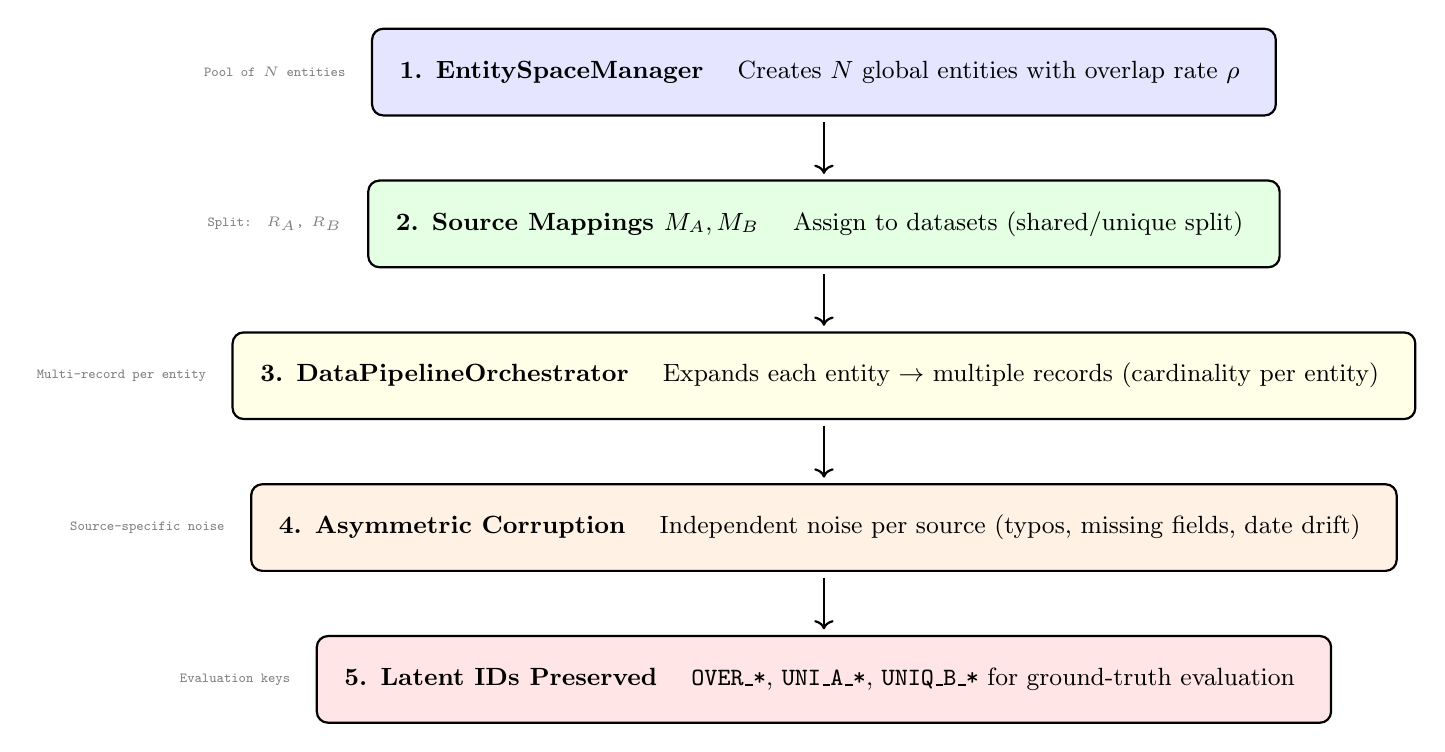
\begin{tikzpicture}[
				node distance=0.8cm,
				every node/.style={font=\small},
				stage/.style={
						draw,
						rectangle,
						rounded corners=4pt,
						minimum width=11cm,
						minimum height=1.1cm,
						align=center,
						thick,
						inner xsep=10pt,
						inner ysep=6pt
					},
				arrow/.style={->, thick, shorten >=2pt, shorten <=2pt}
			]
		% Pipeline stages - vertical stack
		\node[stage, fill=blue!10] (step1) {
			\textbf{1. EntitySpaceManager} \quad Creates $N$ global entities with overlap rate $\rho$
		};
		\node[stage, fill=green!10, below=of step1] (step2) {
			\textbf{2. Source Mappings $M_A, M_B$} \quad Assign to datasets (shared/unique split)
		};
		\node[stage, fill=yellow!10, below=of step2] (step3) {
			\textbf{3. DataPipelineOrchestrator} \quad Expands each entity $\to$ multiple records (cardinality per entity)
		};
		\node[stage, fill=orange!10, below=of step3] (step4) {
			\textbf{4. Asymmetric Corruption} \quad Independent noise per source (typos, missing fields, date drift)
		};
		\node[stage, fill=red!10, below=of step4] (step5) {
			\textbf{5. Latent IDs Preserved} \quad \texttt{OVER\_*}, \texttt{UNI\_A\_*}, \texttt{UNIQ\_B\_*} for ground-truth evaluation
		};

		% Stacked arrows
		\foreach \src/\dst in {step1/step2, step2/step3, step3/step4, step4/step5} {
				\draw[arrow] (\src.south) -- (\dst.north);
			}

		% Side labels showing data flow transformation (Fixed coordinate syntax)
		\node[anchor=east, font=\tiny\ttfamily, text=gray] at ([xshift=-0.2cm]step1.west) {Pool of $N$ entities};
		\node[anchor=east, font=\tiny\ttfamily, text=gray] at ([xshift=-0.2cm]step2.west) {Split: $R_A$, $R_B$};
		\node[anchor=east, font=\tiny\ttfamily, text=gray] at ([xshift=-0.2cm]step3.west) {Multi-record per entity};
		\node[anchor=east, font=\tiny\ttfamily, text=gray] at ([xshift=-0.2cm]step4.west) {Source-specific noise};
		\node[anchor=east, font=\tiny\ttfamily, text=gray] at ([xshift=-0.2cm]step5.west) {Evaluation keys};
	\end{tikzpicture}
	}
	\caption{Synthetic Data Generation Pipeline.
		Vertical stages show the transformation from entity pool $\to$ split datasets $\to$ multi-record expansion $\to$ independent corruption $\to$ ground-truth keys.
		Each stage is a separable, testable component in the codebase.}
	\label{fig:datagen_pipeline}
\end{figure}

The pipeline was designed to easily support customisations at various levels (config, data type, data distributions).

\subsubsection{Configuration (YAML)}
\label{sec:datagen_config}
Key parameters (\texttt{data\_generator/config.yaml}):
\begin{itemize}
	\item \texttt{dataset\_size}: Total global entities $N$.
	\item \texttt{overlap\_percentage}: Fraction $\rho$ of entities present in both datasets.
	\item \texttt{source\_a\_rows\_per\_entity}, \texttt{source\_b\_rows\_per\_entity}: Multiplicity (cardinality) per entity per source.
	\item \texttt{features}: List of $\{ \text{name, type, noise\_params, missing\_rate} \}$.
	      Types: \texttt{categorical} (classes, missing), \texttt{numerical} (Gaussian noise $\sigma$), \texttt{datetime} (Gaussian hours, missing).
	\item \texttt{overlap\_dropout\_frac}: Asymmetric dropout on overlapping portion of B.
\end{itemize}

\subsubsection{Noise Models}
\label{sec:noise_models}
\begin{itemize}
	\item \textbf{Categorical}: Uniform random generation out of \texttt{num\_classes}, missing with \texttt{missing\_rate}.
	\item \textbf{Numerical}: True value $+\ \mathcal{N}(0, \sigma^2)$; missing with \texttt{missing\_rate}.
	\item \textbf{Datetime}: True timestamp $+\ \mathcal{N}(0, \sigma_{\text{hours}}^2)$ hours; missing with \texttt{missing\_rate}.
\end{itemize}

\subsubsection{Latent Event IDs}
Every generated row receives a \texttt{latent\_event\_id}:
\begin{itemize}
	\item \texttt{OVER\_k}: Overlapping entities (same $k$ in A and B $\to$ true match).
	\item \texttt{UNI\_A\_k}: Unique to A.
	\item \texttt{UNIQ\_B\_k}: Unique to B.
\end{itemize}
These enable ground-truth evaluation without manual labelling.


\subsection{Profile Aggregation Engine}
\label{sec:agg_profile_engine}
The profile aggregation engine transforms raw record tables into entity-level profile vectors.
A simplified horizontal flow diagram illustrates the transformation:

\begin{figure}[htbp]
	\centering
	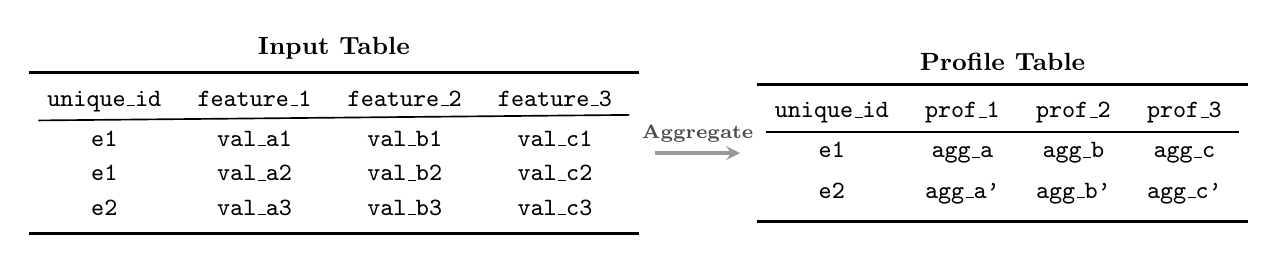
\begin{tikzpicture}[
			node distance=1.0cm,
			every node/.style={font=\small},
			tableTitle/.style={font=\small\bfseries},
			% Compact stealth arrows
			arrow/.style={->, >=stealth, thick, line width=1.2pt, color=gray!80, shorten >=6pt, shorten <=6pt}
		]

		% --- INPUT TABLE ---
		\matrix [matrix of nodes, nodes={align=left, inner sep=3pt}, row sep=1pt, column sep=4pt] (inputTable) {
			\rowcolor{tableHeader} \textbf{\texttt{unique\_id}} & \textbf{\texttt{feature\_1}} & \textbf{\texttt{feature\_2}} & \textbf{\texttt{feature\_3}} \\
			\texttt{e1} & \texttt{val\_a1} & \texttt{val\_b1} & \texttt{val\_c1} \\
			\rowcolor{tableRowEven} \texttt{e1} & \texttt{val\_a2} & \texttt{val\_b2} & \texttt{val\_c2} \\
			\texttt{e2} & \texttt{val\_a3} & \texttt{val\_b3} & \texttt{val\_c3} \\
		};
		% Crisp top/bottom borders
		\draw[line width=1.1pt] (inputTable.north west) -- (inputTable.north east);
		\draw[line width=0.6pt] (inputTable-1-1.south west) -- (inputTable-1-4.south east);
		\draw[line width=1.1pt] (inputTable.south west) -- (inputTable.south east);
		\node[tableTitle, above=0.05cm of inputTable] (inputTitle) {Input Table};

		% --- OUTPUT PROFILE TABLE ---
		\matrix [matrix of nodes, nodes={align=left, inner sep=3pt}, row sep=1pt, column sep=4pt, right=1.5cm of inputTable] (outputTable) {
			\rowcolor{tableHeader} \textbf{\texttt{unique\_id}} & \textbf{\texttt{prof\_1}} & \textbf{\texttt{prof\_2}} & \textbf{\texttt{prof\_3}} \\
			\texttt{e1} & \texttt{agg\_a} & \texttt{agg\_b} & \texttt{agg\_c} \\
			\rowcolor{tableRowEven} \texttt{e2} & \texttt{agg\_a'} & \texttt{agg\_b'} & \texttt{agg\_c'} \\
		};
		% Crisp top/bottom borders matching the input table exactly
		\draw[line width=1.1pt] (outputTable.north west) -- (outputTable.north east);
		\draw[line width=0.6pt] (outputTable-1-1.south west) -- (outputTable-1-4.south east);
		\draw[line width=1.1pt] (outputTable.south west) -- (outputTable.south east);
		\node[tableTitle, above=0.05cm of outputTable] (outputTitle) {Profile Table};

		% --- DIRECT FLOW ARROW WITH LABEL ---
		\draw[arrow] (inputTable.east) -- node[above, font=\scriptsize\bfseries, color=black!70] {Aggregate} (outputTable.west);

	\end{tikzpicture}
	\caption{Horizontal flow of the profile aggregation engine: raw records are grouped by entity identifier and transformed into fixed‑dimensional profile vectors.}
	\label{fig:profile_agg_flow}
\end{figure}

The full implementation resides in the \texttt{em/aggregation/} package. It uses a \texttt{ProcessorRegistry} to map feature types to \texttt{ColumnProcessor} subclasses, and an \texttt{Aggregator} that coordinates multiple processors, builds vocabularies, applies aggregation functions, and runs post‑processors.

\subsection{Splink Configuration Overview}
\label{sec:splink_config}
The Entity Matching pipeline uses the Splink library for probabilistic record linkage.
All synthetic datasets share identical comparison logic; only dataset paths and resource parameters vary.
Notebooks with real datasets reuse the same structure with domain‑specific field mappings.

Supported comparison functions include:
\begin{itemize}
	\item Basic Splink levels: \texttt{NullLevel}, \texttt{ExactMatchLevel}, \texttt{ElseLevel}.
	\item Binned levels: \texttt{PercentageDifferenceLevel}, \texttt{WithinNDaysLevel}, \texttt{JaroWinklerLevel}.
	\item Custom comparisons via SQL expressions (e.g., for set similarities, range overlap).
\end{itemize}

The core workflow follows the Splink transaction demo pattern:
\begin{enumerate}
	\item Define comparison levels for each field.
	\item Specify blocking rules as SQL predicates.
	\item Train the model via expectation‑maximisation (EM) using a fixed schedule of blocking rules.
	\item Generate predictions and evaluate against known latent IDs.
\end{enumerate}

Full code listings are in the respective notebooks mentioned by the report.

\subsection{Blocking Rules Design}
\label{sec:blocking_rules}
Blocking rules are supplied as an array of SQL predicates to the argument \texttt{blocking\_rules\_to\_generate\_predictions}.
Each rule targets a different matching signal (e.g., categorical equality, numerical proximity, temporal proximity) and their union bounds recall while reducing the comparison space.
Example predicates (for synthetic data) are of the form:
\begin{itemize}
	\item \texttt{l.categorical = r.categorical OR l.categorical IS NULL OR r.categorical IS NULL}
	\item \texttt{strftime(l.datetime\_noisy, '\%Y\%m') = strftime(r.datetime\_noisy, '\%Y\%m') OR l.datetime\_noisy IS NULL OR r.datetime\_noisy IS NULL}
	\item \texttt{(ABS(l.numerical\_noisy - r.numerical\_noisy) / NULLIF(CASE WHEN l.numerical\_noisy > r.numerical\_noisy THEN l.numerical\_noisy ELSE r.numerical\_noisy END, 0)) < 0.25 OR l.numerical\_noisy IS NULL OR r.numerical\_noisy IS NULL}
\end{itemize}

Full code listings are in the respective notebooks mentioned by the report.

\subsection{EM Training Schedule}
\label{sec:em_training}
Parameter estimation proceeds via a fixed sequence of expectation‑maximisation steps, each using a different blocking rule to estimate m‑probabilities for the remaining comparisons.
The schedule begins with estimating the global prior from strict rules, then estimates u‑probabilities via random sampling, followed by EM rounds that alternate blocking columns to identify all m‑probabilities.

Full code listings are in the respective notebooks mentioned by the report.


% ============================================================
% 4. Experimental Methodology
% ============================================================
% ============================================================
% 4. Experimental Methodology
% ============================================================
\section{Experimental Methodology}
\label{sec:methodology}

\subsection{Datasets}
\label{sec:datasets}

The naming for the datasets are completely arbitrary, and hold little meaning towards the actual config and structure of the datasets.

\begin{table}[htbp]
	\centering
	\caption{Datasets Used in Experiments}
	\label{tab:datasets}
	% Save standard booktabs spacing to prevent text clipping
	\newlength{\oldaboverulesep}
	\newlength{\oldbelowrulesep}
	\setlength{\oldaboverulesep}{\aboverulesep}
	\setlength{\oldbelowrulesep}{\belowrulesep}
	
	% Set spacing to zero inside colored rows to fix the background overlap
	\setlength{\aboverulesep}{0pt}
	\setlength{\belowrulesep}{0pt}

	\begin{tabular}{llcccc}
		\toprule
		\rowcolor{gray!15} \textbf{Name} & \textbf{Type} & \textbf{Entities} & \textbf{Overlap} & \textbf{Cardinality} & \textbf{Source} \\
		\midrule
		% Restore normal spacing for the rest of the table
		\noalign{\setlength{\aboverulesep}{\oldaboverulesep}\setlength{\belowrulesep}{\oldbelowrulesep}}
		\texttt{base}         & Synthetic     & 50                & 30\%             & 70/80                & \texttt{generate\_data.py} \\
		\texttt{smallest}          & Synthetic     & 50                & 10\%             & 35/45                & \texttt{generate\_data.py} \\
		\texttt{low\_card}        & Synthetic     & 100               & 10\%             & 18/12                  & \texttt{generate\_data.py} \\
		\texttt{o50}              & Synthetic     & 50             & 50\%             & 30/35              & \texttt{generate\_data.py} \\
		\texttt{MusicBrainz}      & Real  & ~3,900 / ~3,800   & ~27\%            & Multi / Multi        & Public (MusicBrainz)       \\
		\bottomrule
	\end{tabular}
\end{table}

\subsection{Evaluation Protocol}
\label{sec:evaluation_protocol}

\subsubsection{Synthetic Data: Ground-Truth Available}
Since \texttt{latent\_event\_id} is preserved, we construct a clerical labels table:
\begin{enumerate}
	\item Merge predictions with ground truth on \texttt{latent\_event\_id\_l == latent\_event\_id\_r}.
	\item Compute TP, FP, FN, TN at each probability threshold.
	\item Derive Precision, Recall, $F_1$, Accuracy.
	\item Select optimal threshold via maximum $F_1$.
\end{enumerate}

\subsubsection{Public Data: No Ground Truth}
For MusicBrainz, we rely on:
\begin{itemize}
	\item \textbf{Blocking recall bounds}: Theoretical upper bound on recall from blocking rule coverage.
	\item \textbf{Precision/Recall estimation}: Using the \splink{} accuracy analysis with a small manual clerical sample (if available) or synthetic proxy.
	\item \textbf{Stability checks}: Consistency of match weights across \emalgo{} rounds; separation of match/non-match weight distributions.
\end{itemize}

\subsubsection{Metrics}
\label{sec:metrics}
\begin{gather}
	\text{Precision} = \frac{TP}{TP + FP}                                                                    \\
	\text{Recall} = \frac{TP}{TP + FN}                                                                    \\
	F_1 = 2 \cdot \frac{\text{Precision} \cdot \text{Recall}}{\text{Precision} + \text{Recall}} \\
	\text{Accuracy} = \frac{TP + TN}{TP + FP + FN + TN}
\end{gather}


For global aggregation experiments, we also report \textbf{global entity-level} metrics after aggregation (matching on \texttt{global\_entity\_id}).

\subsection{Baselines and Ablations}
\label{sec:baselines}

\begin{description}
	\item[\textbf{Normalised Aggregation}] Mean probability per global pair; threshold.
	\item[\textbf{Noisy-OR Aggregation}] Probabilistic union; threshold.
	\item[\textbf{Max Aggregation}] Max probability per global pair; threshold.
	\item[\textbf{Vector-Space Aggregation}] Profile vectors, second \splink{} layer (\Cref{sec:profile_aggregation}).
	\item[\textbf{Data Config Variants}] Varying data structure.
\end{description}

\subsection{Computational Environment}
\label{sec:compute_env}
\begin{itemize}
	\item DuckDB in-memory with 24GB memory limit, spill to disk.
	\item \splink{} 4.x (Python-native).
	\item Python 3.11, pandas, numpy, scikit-learn for metrics.
	\item Runtime: Local layer prediction ~1-20s depending on config; global aggregation negligible.
\end{itemize}


% ============================================================
% 5. Experimental Results \& Discussion
% ============================================================
% ============================================================
% 5. Experimental Results \& Discussion
% ============================================================
\section{Experimental Results \& Discussion}
\label{sec:results}

\subsection{Experiment 1: \texttt{base} Synthetic Dataset - \texttt{splink\_local\_demo.ipynb}}
\label{sec:exp_smaller}
\subsubsection{Dataset Description}
This dataset consists of two tables with approximately 3,300 and 3,700 records, generated with 50 entities each, 30\% overlap, and 70/80 records per entity (A/B). It serves as our primary artificial dataset for evaluating the Splink pipeline while maintaining computational tractability.
\subsubsection{Blocking Rules Design}
\label{sec:blocking_rules_exp1}
The blocking rules target orthogonal signals to bound recall while reducing the comparison space. Each rule is a disjunctive condition that allows matches when the attribute agrees or when data is missing on either side.
The four blocking rules used are:
\begin{enumerate}
    \item Categorical equality or missing
    \item Numerical within 25\% or missing
    \item Date within +1 day or missing
    \item Date within -1 day or missing
\end{enumerate}
(See notebooks for the exact SQL predicates.)
\subsubsection{Comparison Levels}
\label{sec:comparison_levels_exp1}
Each field is modeled with a \texttt{CustomComparison} using binned levels that capture gradations of similarity. The levels are chosen to reflect the noise models used in synthetic data generation.

For the numerical field, we use PercentageDifferenceLevel bins at 5\%, 10\%, 25\%, and 50\%.
For the categorical field, we use ExactMatchLevel.
For the datetime field, we use WithinNDaysLevel bins at 0 days (same day), 1 day, and 5 days.
For the textual name fields, we use Jaro-Winkler bins at 0.8, 0.5, 0.3.
(See notebooks for full specification.)
\subsubsection{Local Pairwise Matching Results}
\begin{itemize}
    \item \textbf{Match weight chart:} Figure~\ref{fig:match_weights_smaller} displays the m‑probability, u‑probability, bayes factor, and log2 bayes factor for each comparison level. This chart reveals which comparisons contribute most to the match weight.
    \item \textbf{Threshold selection curve:} Figure~\ref{fig:threshold_curve_smaller} shows precision, recall, and F1 score as functions of the match probability threshold. The curve illustrates the trade-off between precision and recall across different threshold values.
\end{itemize}

% Add figures for the small dataset
\begin{figure}[H]
    \centering
    \includegraphics[width=\textwidth]{images/splink_local_demo/match_weights_chart.png}
    \caption{Match weights chart showing m-probability, u-probability, bayes factor, and log2 bayes factor for each comparison level in the small synthetic dataset.}
    \label{fig:match_weights_smaller}
\end{figure}

\begin{figure}[H]
    \centering
    \includegraphics[width=\textwidth]{images/splink_local_demo/threshold_curve.png}
    \caption{Threshold selection curve showing precision, recall, and F1 score as functions of the match probability threshold for the small synthetic dataset. The curve illustrates the trade-off between precision and recall across different threshold values.}
    \label{fig:threshold_curve_smaller}
\end{figure}

\subsubsection{Threshold Selection and Results}
The intent behind threshold selection in these experiments is not to find an \textit{optimal} threshold, but to ensure as large a \textbf{range of values} that would be considered \textit{acceptable performances}. This is identical to spreading the gap between probabilities. 

\subsubsection{Local matching - Discussion}
We notice from the match weights that the model seems to lean towards \textit{heavy penalties} on mismatches over rewarding matches. Mismatches in numerical columns and the datetime are immediately penalised heavily. 

Intuitively - these comparison-level mismatches are considered as effectively \textit{equivalent} to a complete record mismatch.
\subsubsection{Blocking Efficiency}
With the same blocking rules, the number of comparisons after blocking is reduced from the full cartesian product of ~3.48 million to 1,394,506.

\subsubsection{Local-to-Global Aggregation Analysis}
We apply local-to-global aggregation techniques to the base dataset by constructing entity pairs and computing various aggregation strategies that align with the theoretical framework taxonomy in Section~\ref{sec:framework}. Specifically, we implement:
\begin{itemize}
    \item \textbf{Match density} (\texttt{sum\_p}) - see Section~\ref{sec:agg_functions}
    \item \textbf{Max-Over-Partitions} (\texttt{max\_w}) - see Section~\ref{sec:agg_functions}
    \item \textbf{Noisy-OR} (\texttt{score\_noisy\_or}) - see Section~\ref{sec:agg_functions}
    \item \textbf{Vector-Space-inspired} (\texttt{top\_3\_mean\_w}, \texttt{score\_softmax\_p}) - see Section~\ref{sec:agg_functions}
    \item \textbf{Weighted Jaccard} (\texttt{weighted\_jaccard}) - see Section~\ref{sec:agg_functions}
    \item \textbf{Weighted Overlap} (\texttt{weighted\_overlap}) - see Section~\ref{sec:agg_functions}
    \item \textbf{Score-probability expected ratio} (\texttt{score\_prob\_expected\_ratio}) - see Section~\ref{sec:agg_functions}
\end{itemize}

\begin{figure}[H]
    \centering
    \includegraphics[width=\textwidth]{images/splink_local_demo/aggregation_score_heatmaps.png}
    \caption{Aggregation score heatmaps showing various aggregation strategies (sum, max, top-k mean, noisy-or, softmax, match density, weighted Jaccard, weighted overlap, score-probability expected ratio) between entities in the base synthetic dataset, demonstrating the theoretical framework's aggregation functions in practice.}
    \label{fig:aggregation_heatmaps_base}
\end{figure}

\begin{figure}[H]
    \centering
    \includegraphics[width=\textwidth]{images/splink_local_demo/threshold_evaluation_binned.png}
    \caption{Threshold evaluation curves (precision, recall, F1 binned into equal-width intervals) for each aggregation strategy on the base synthetic dataset, demonstrating performance across the theoretical framework's aggregation functions.}
    \label{fig:threshold_evaluation_base}
\end{figure}

% Discussion of results would go here, comparing baseline vs aggregation performance
\subsubsection{Global Aggregation - Discussion}
We term the threshold curves for each aggregation function as \textit{profiles}. We note that for a few of the profiles, namely the weighted Jaccard and the weighted overlap, the profile is generally stable - the recall and precision are not volatile. Furthermore, the scores on these functions are also exceptional - at recall 1.0 and precision 1.0 for a large range of these values.

\subsection{Experiment 2: Synthetic Dataset Variants}
\label{sec:exp_variants}
To understand how specific dataset characteristics affect matching quality and computational efficiency, we created several variants of the synthetic dataset by modifying single parameters while keeping the Splink configuration constant. This allows us to isolate the impact of each factor.
\subsubsection{Variant Overview}
\begin{itemize}
    \item \texttt{smallest}: This dataset consists of two tables with approximately 3,300 and 3,700 records, generated with 50 entities each, 10\% overlap, and 35/45 records per entity.
    \item \texttt{low\_card}: 100 entities each, 10\% overlap, 18/12 records per entity (low intra-entity variation)
    \item \texttt{o50}: 50 entities each, 50\% overlap, 30/35 records per entity
\end{itemize}
\subsubsection{Configuration}
All variants use the identical Splink configuration as Experiment~1 (same four blocking rules and three comparisons).
\subsubsection{Results Summary}
Each variant's results and metrics are to be extracted from their respective notebooks:
\begin{itemize}
    \item \texttt{splink\_local\_smallest.ipynb} (smallest)
    \item \texttt{splink\_low\_card.ipynb} (low\_card)
    \item \texttt{splink\_o50.ipynb} (o50)
\end{itemize}

\subsubsection{Intent}
The variant experiments reveal how different dataset characteristics influence the EM algorithm's convergence and the final matching quality:
\begin{itemize}
    \item \textbf{Overlap percentage}: Higher overlap (as in \texttt{o50}) introduces an error in the estimated prior - we show that selection via \textit{ranking} still maintains performance.
    \item \textbf{Entity count}: Increasing entities (as in \texttt{smallest} against \texttt{base}) improves estimation stability but increases computational cost.
    \item \textbf{Cardinality}: Higher intra-entity variation (as in \texttt{base} against \texttt{low\_card}) improves discrimination at every level.
\end{itemize}

\subsubsection{smallest Variant}
\label{sec:exp_smallest}
\paragraph{Dataset Description}
The smallest variant has 50 entities each, 10\% overlap, and cardinality 35/45 per entity.

\paragraph{Results}
Figures~\ref{fig:match_weights_smallest} and~\ref{fig:threshold_curve_smallest} show the match weights and threshold selection curve for this variant.

\begin{figure}[H]
    \centering
    \includegraphics[width=\textwidth]{images/splink_local_smallest/match_weights_chart.png}
    \caption{Match weights chart for the smallest variant (50 entities, 10\% overlap, 35/45 cardinality).}
    \label{fig:match_weights_smallest}
\end{figure}

\begin{figure}[H]
    \centering
    \includegraphics[width=\textwidth]{images/splink_local_smallest/threshold_curve.png}
    \caption{Threshold selection curve for the smallest variant.}
    \label{fig:threshold_curve_smallest}
\end{figure}

\subsubsection{Local-to-Global Aggregation Analysis}
We apply identical local-to-global aggregation techniques to the smallest variant dataset.

\begin{figure}[H]
    \centering
    \includegraphics[width=\textwidth]{images/splink_local_smallest/aggregation_score_heatmaps.png}
    \caption{Aggregation score heatmaps showing various aggregation strategies (sum, max, top-k mean, noisy-or, softmax, match density, weighted Jaccard, weighted overlap, score-probability expected ratio) between entities in the smallest variant dataset, demonstrating the theoretical framework's aggregation functions in practice.}
    \label{fig:aggregation_heatmaps_smallest}
\end{figure}

\begin{figure}[H]
    \centering
    \includegraphics[width=\textwidth]{images/splink_local_smallest/threshold_evaluation_binned.png}
    \caption{Threshold evaluation curves (precision, recall, F1 binned into equal-width intervals) for each aggregation strategy on the smallest variant dataset, demonstrating performance across the theoretical framework's aggregation functions.}
    \label{fig:threshold_evaluation_smallest}
\end{figure}

\paragraph{Discussion}
We notice that without the textual name columns, our model performs significantly worse on pairwise matching. Most of these comparison matches are still susceptible to coincidental matches, which result in lower match weights even on matches.

We penalise heavily, as expected, on mismatches as we have previously, but the lack of more
discriminatory columns affected local matching significantly.

However, when extended to the global aggregate scores, our performance, while indeed poorer,
still retains a satisfiable level of stability. In particular, weighted Jaccard and weighted overlaps retain similar profiles to that of the base variant.

\subsubsection{low\_card Variant}
\label{sec:exp_low_card}
\paragraph{Dataset Description}
The low\_card variant has 100 entities each, 10\% overlap, and cardinality 18/12 per entity (low intra-entity variation).

\paragraph{Results}
Figures~\ref{fig:match_weights_low_card} and~\ref{fig:threshold_curve_low_card} show the match weights and threshold selection curve for this variant.

\begin{figure}[H]
    \centering
    \includegraphics[width=\textwidth]{images/splink_local_low_card/match_weights_chart.png}
    \caption{Match weights chart for the low\_card variant (100 entities, 10\% overlap, 18/12 cardinality).}
    \label{fig:match_weights_low_card}
\end{figure}

\begin{figure}[H]
    \centering
    \includegraphics[width=\textwidth]{images/splink_local_low_card/threshold_curve.png}
    \caption{Threshold selection curve for the low\_card variant.}
    \label{fig:threshold_curve_low_card}
\end{figure}

\subsubsection{Local-to-Global Aggregation Analysis}
We apply identical local-to-global aggregation techniques to the low\_card variant dataset.

\begin{figure}[H]
    \centering
    \includegraphics[width=\textwidth]{images/splink_local_low_card/aggregation_score_heatmaps.png}
    \caption{Aggregation score heatmaps showing various aggregation strategies (sum, max, top-k mean, noisy-or, softmax, match density, weighted Jaccard, weighted overlap, score-probability expected ratio) between entities in the low\_card variant dataset, demonstrating the theoretical framework's aggregation functions in practice.}
    \label{fig:aggregation_heatmaps_low_card}
\end{figure}

\begin{figure}[H]
    \centering
    \includegraphics[width=\textwidth]{images/splink_local_low_card/threshold_evaluation_binned.png}
    \caption{Threshold evaluation curves (precision, recall, F1 binned into equal-width intervals) for each aggregation strategy on the low\_card variant dataset, demonstrating performance across the theoretical framework's aggregation functions.}
    \label{fig:threshold_evaluation_low_card}
\end{figure}

\paragraph{Discussion}
We find that the previous discussion from \ref{sec:exp_smallest} finds its extremes here. Most comparisons are weakly discriminatory in nature, and we find that the model is unable to discriminate matches from noise.

Cardinality contributes to the discriminatory effect of Fellegi-Sunter. Here, we only have a total of 8 possible comparison vectors across the entire pair space, which creates little granularity for the necessary discriminatory effect.

This instability extends to the aggregation functions as well - the profiles on most, if not all, of the aggregation functions do not seem viable for stable use.

\subsubsection{o50 Variant}
\label{sec:exp_o50}
\paragraph{Dataset Description}
The o50 variant has 50 entities each, 50\% overlap, and cardinality 30/35 per entity (high prior match probability).

\paragraph{Results}
Figures~\ref{fig:match_weights_o50} and~\ref{fig:threshold_curve_o50} show the match weights and threshold selection curve for this variant.

\begin{figure}[H]
    \centering
    \includegraphics[width=\textwidth]{images/splink_local_o50/match_weights_chart.png}
    \caption{Match weights chart for the o50 variant (50 entities, 50\% overlap, 30/35 cardinality).}
    \label{fig:match_weights_o50}
\end{figure}

\begin{figure}[H]
    \centering
    \includegraphics[width=\textwidth]{images/splink_local_o50/threshold_curve.png}
    \caption{Threshold selection curve for the o50 variant.}
    \label{fig:threshold_curve_o50}
\end{figure}

\subsubsection{Local-to-Global Aggregation Analysis}
We apply identical local-to-global aggregation techniques to the o50 variant dataset.

\begin{figure}[H]
    \centering
    \includegraphics[width=\textwidth]{images/splink_local_o50/aggregation_score_heatmaps.png}
    \caption{Aggregation score heatmaps showing various aggregation strategies (sum, max, top-k mean, noisy-or, softmax, match density, weighted Jaccard, weighted overlap, score-probability expected ratio) between entities in the o50 variant dataset, demonstrating the theoretical framework's aggregation functions in practice.}
    \label{fig:aggregation_heatmaps_o50}
\end{figure}

\begin{figure}[H]
    \centering
    \includegraphics[width=\textwidth]{images/splink_local_o50/threshold_evaluation_binned.png}
    \caption{Threshold evaluation curves (precision, recall, F1 binned into equal-width intervals) for each aggregation strategy on the o50 variant dataset, demonstrating performance across the theoretical framework's aggregation functions.}
    \label{fig:threshold_evaluation_o50}
\end{figure}

\paragraph{Discussion}
We find that the local matching performance of the model is somewhat similar to that of the smallest variant - albeit more granular. We attribute this step up due to having more ground truths.

We notice that the effect of wrongly estimating the recall when estimating the prior has little
noticeable effects on model performance.

This is further shown when we extend to the aggregation functions - some of the threshold curves
retain their profile, namely the weighted Jaccard and weighted overlap.

\subsection{Experiment 3: Public Dataset Validation: MusicBrainz}
\label{sec:exp_musicbrainz}
\subsubsection{Description}
This experiment can be found in \texttt{splink\_music.ipynb} and \texttt{splink\_music\_agg.ipynb}.

Two snapshots of the MusicBrainz dataset (catalog 3 vs catalog 5), each with approximately 3,900 and 3,800 artists (multi-record per entity). Attributes: title (set), album (set), track number (set), length (numeric), language (set), year (set).
\subsubsection{Configuration}
We block on at least one intersecting track number; comparison levels include soft Jaccard on title/album, Simpson on track number, year overlap, and numerical range overlap on length. The EM algorithm converges with 4 training rules.

Specifically, blocking rules are:
\begin{enumerate}
    \item Same Artist AND Same Track Number
    \item Same Track Number AND Same Title Prefix (Extended to 6 characters)
    \item Exact Artist Match AND Title Prefix Match (first 4 characters)
\end{enumerate}
Comparison levels include:
\begin{itemize}
    \item Artist: Null, ExactMatch, JaroWinkler (threshold 0.88), Else
    \item Title Lexical: Null, ExactMatch, Prefix condition (title\_l LIKE title\_r || '%' OR title\_r LIKE title\_l || '%'), JaroWinkler (0.90), Else
    \item Title Tokens: Null, Jaccard (0.80), Jaccard (0.55), Else
    \item Album: Null, ExactMatch, Album truncation match, Else
    \item Length: Null, Length within 15\%, Length within 40\%, Else
    \item Year: Standardized year list check using clean native DuckDB list operations (levels to be defined)
    \item Track Number: ExactMatch
\end{itemize}

\subsubsection{Blocking Efficiency}
The Cartesian product yields 15,028,728 comparisons. After applying the three blocking rules, the number of comparisons is reduced to 1,471 (a reduction of >99.99\%). 

\paragraph{Pre local-to-global matching}
Figures~\ref{fig:match_weights_music} and~\ref{fig:threshold_curve_music} show the match weights and threshold selection curve for the baseline Splink model (no aggregation).

\begin{figure}[H]
    \centering
    \includegraphics[width=\textwidth]{images/splink_music/match_weights.png}
    \caption{Match weights chart showing m-probability, u-probability, bayes factor, and log2 bayes factor for each comparison level in the MusicBrainz dataset.}
    \label{fig:match_weights_music}
\end{figure}

\begin{figure}[H]
    \centering
    \includegraphics[width=\textwidth]{images/splink_music/local_threshold_curve_old.png}
    \caption{Threshold selection curve showing precision, recall, and F1 score as functions of the match probability threshold for the baseline Splink model on the MusicBrainz dataset.}
    \label{fig:threshold_curve_music}
\end{figure}
\subsubsection{Local-to-Global Aggregation Analysis}
We apply local-to-global aggregation techniques to the MusicBrainz dataset by constructing entity pairs and computing various aggregation strategies that align with the theoretical framework taxonomy in Section~\ref{sec:framework}. Specifically, we implement:
\begin{itemize}
    \item \textbf{Match density} (\texttt{sum\_p}) - see Section~\ref{sec:agg_functions}
    \item \textbf{Max-Over-Partitions} (\texttt{max\_w}) - see Section~\ref{sec:agg_functions}
    \item \textbf{Noisy-OR} (\texttt{score\_noisy\_or}) - see Section~\ref{sec:agg_functions}
    \item \textbf{Score-probability expected ratio} (\texttt{score\_prob\_expected\_ratio}) - see Section~\ref{sec:agg_functions}
\end{itemize}
\begin{figure}[H]
    \centering
    \includegraphics[width=\textwidth]{images/splink_music/threshold_curve.png}
    \caption{Threshold evaluation curves (precision, recall, F1 binned into equal-width intervals) for each aggregation strategy on the MusicBrainz dataset, demonstrating performance across the theoretical framework's aggregation functions.}
    \label{fig:threshold_evaluation_music}
\end{figure}

\subsubsection{Discussion}
The ground truths are established as a match on the artist column, acknowledging that some artists don't actually have exact matches due to name typos (see Annex \ref{annex:artist_matching} for details on how this affects precision and recall). Under specific assumptions, we establish that precision is a definite lower bound, but recall is bounded to a fair estimate, and is likely an overestimation.

The MusicBrainz results confirm that the \splink{} pipeline, and the aggregation framwork, generalizes to real-world, multi-record entity resolution scenarios. Local-to-global aggregation further enhances matching performance by leveraging distributional properties of match probabilities across record pairs.

We then discuss the stability of the global aggregation profiles, suggesting viability in using \splink{} for unsupervised matching in similar scenarios.

\subsection{Experiment 4: Behavioural Aggregation Experiments}
\label{sec:exp_aggregation}
\subsubsection{Description}
This set of experiments builds profile vectors per global entity using numerical aggregates (mean, min, max of length) and categorical sets (title, album, language) converted to frequency vectors, then applies \splink{} to compare these profile vectors. We evaluate this approach on both our synthetic datasets (base, and low\_card) and the MusicBrainz dataset.

\subsubsection{Configuration}
The blocking rules and comparison levels are defined in the notebook they reference. General rule design concerning strictness of the blocking rules were applied. 

The set comparisons are based on the attribute types (numerical, categorical, etc.) and are designed to capture similarity in the same way as the baseline experiments, but applied to the profile variables.

\paragraph{Base Dataset - \texttt{agg\_eg\_normal.ipynb}}
In this experiment, for simplicity, we do not use
textual set-comparisons. We leverage on two key comparisons: magnitude-normalised cosine vectors, as well as the "bag" of tokens for each entity
\subparagraph{Match weights}
We observe that the model relies extremely heavily on penalising poor matches - the likelihood of finding an exact match on these set similarity functions become much less likely.

We can build an intuition around this - the profiles of these entities are vastly different: the cosine vectors, as well as the "bag" of contents, are different. 

Good matches can still be found by coincidence, but bad matches are immediately indicative, and equivalent, of a non-match overall.
\begin{figure}[H]
    \centering
    \includegraphics[width=\textwidth]{images/splink_behaviour_base/match_weights.png}
    \caption{Match weights chart for the base variant dataset.}
    \label{fig:match_weights_base}
\end{figure}

\subparagraph{Threshold selection curve}
The profile here is extremely stable, and suggests promising results.
\begin{figure}[H]
    \centering
    \includegraphics[width=\textwidth]{images/splink_behaviour_base/threshold_curve.png}
    \caption{Threshold selection curve for the base variant dataset. The orange dotted curve is recall, blue dashed-line is precision. Green bold line is F1.}
    \label{fig:threshold_curve_base}
\end{figure}


\paragraph{Low-card Dataset - \texttt{agg\_eg.ipynb}}
We attempt find a better solution to global entity matching in profile aggregation with the low\_card dataset.

\subparagraph{Match weights}
The discriminatory factors on some of the set comparisons are strong - the model is able to pick up on mismatches between entities.
\begin{figure}[H]
    \centering
    \includegraphics[width=\textwidth]{images/splink_behaviour_low_card/match_weights.png}
    \caption{Match weights chart for the low\_card variant dataset.}
    \label{fig:match_weights_low_card}
\end{figure}

\subparagraph{Threshold selection curve}
The profile is much more stable than observed from aggregation attempts.
\begin{figure}[H]
    \centering
    \includegraphics[width=\textwidth]{images/splink_behaviour_low_card/threshold_curve.png}
    \caption{Threshold selection curve for the low\_card variant dataset. The orange dotted curve is recall, blue dashed-line is precision. Green bold line is F1.}
    \label{fig:threshold_curve_low_card}
\end{figure}

\paragraph{MusicBrainz Dataset - \texttt{agg\_music.ipynb}}
We attempt to extend this approach to the music dataset, to explore its viability on real world datasets.
\subparagraph{Match weights}
We find that the model penalises only soft Simpson mismatches (< 0.4) to a high degree.

Text based comparisons are difficult to configure in nature - however, the crux of the problem is that there are no indicative mismatches. We discuss this later.
\begin{figure}[H]
    \centering
    \includegraphics[width=\textwidth]{images/splink_behaviour_music/match_weights.png}
    \caption{Match weights chart for the MusicBrainz dataset.}
    \label{fig:match_weights_music}
\end{figure}

\subparagraph{Threshold selection curve}
The lack of confident matches (or, indicative mismatches) propogates to instability in the threshold profile.
\begin{figure}[H]
    \centering
    \includegraphics[width=\textwidth]{images/splink_behaviour_music/threshold_curve.png}
    \caption{Threshold selection curve for the MusicBrainz dataset. The orange dotted curve is recall, blue dashed-line is precision. Green bold line is F1.}
    \label{fig:threshold_curve_music}
\end{figure}

\subsubsection{Discussion}
The core approach in behavioural aggregation is in \textit{profile matching}. In our synthetic dataset, the columns generated per row refer to a specific "event" - each of which has a unique, independent, distribution behind their generation.

In the MusicBrainz dataset, the individual records are \textit{songs} - which skews the distribution of certain columns to a significant degree. The track numbers often WILL contain numbers from 1-5, and song duration distributions are often similar (2-4 minutes in length). These profiles are no longer unique - since every row is a song, every row's profile would be that \textit{of} a song.

Most columns, in this case, provide effectively \textbf{no information} whatsoever to a profile match.

We find that the framework, can, and often does well, match profiles - but only in the specific case that entities are \textit{uniquely profile-able}.

\subsection{Experiment 5: Hierarchical 2-Layer Splink Approach}
\label{sec:exp_hierarchical}
\subsubsection{Description}
This experiment explores a hierarchical approach where we first apply local \splink{} matching to generate match probabilities, then use these probabilities as features in a second-layer Fellegi-Sunter model. We demonstrate this approach using the low\_card variant as an example.

\subsubsection{Configuration}
For the first layer, we use the identical Splink configuration as Experiment~1 (same four blocking rules and three comparisons). The match probabilities from the first layer are then used as input features for the second-layer Splink model, which employs a simpler configuration focused on learning weights for combining these probabilistic signals.

\subsubsection{Results}
From \texttt{splink\_low\_card.ipynb}, we extract:
\begin{itemize}
    \item Hierarchical 2-layer Splink results: threshold curves showing precision, recall, and F1 scores across threshold values
\end{itemize}

\begin{figure}[H]
   \centering
   \includegraphics[width=\textwidth]{images/splink_local_low_card/layer_2_weights.png}
   \caption{Match weights chart showing m-probability, u-probability, bayes factor, and log2 bayes factor for each comparison level in the hierarchical 2-layer Splink approach on the low\_card variant.}
   \label{fig:hierarchical_match_weights_low_card}
\end{figure}

\begin{figure}[H]
   \centering
   \includegraphics[width=\textwidth]{images/splink_local_low_card/layer_2_curve.png}
   \caption{Threshold selection curve showing precision, recall, and F1 score as functions of the match probability threshold for the hierarchical 2-layer Splink approach on the low\_card variant. The curve illustrates the trade-off between precision and recall across different threshold values.}
   \label{fig:hierarchical_threshold_curve_low_card}
\end{figure}


\subsubsection{Discussion}
\begin{itemize}
    \item \textbf{Polarising Effect}: As expected from the theoretical discussion in Section~\ref{sec:framework}, the second layer exhibits polarising behaviour - the learned weights tend to extreme values, acting as ``kingmakers'' that dominantly select certain aggregation functions over others rather than learning balanced combinations.
    \item \textbf{Weight Interpretability vs. Practical Utility}: While the second-layer weights are explainable and indicate which aggregation functions the model considers most predictive, this extreme weighting renders the approach currently unviable for practical use (or, a viable dataset is yet to be found for this approach). The model effectively reduces to selecting a single dominant aggregation function rather than learning a nuanced combination.
    \item \textbf{Generalisation Challenge}: This behaviour highlights the need for further research into aggregation functions that are more generalisable and robust across different dataset characteristics. Fixed aggregation strategies may currently provide more stable performance than learned hierarchical weights.
    \item \textbf{Comparison to Direct Aggregation}: Initial exploration suggests that direct aggregation methods (sum, max, top-k mean, noisy-or, softmax) often provide more consistent and interpretable results than the hierarchical approach, which tends to overfit to the training signal.
    \item \textbf{Scalability Considerations}: While training two sequential Splink models increases computational complexity, the primary limitation is not computational but methodological - the hierarchical approach as currently formulated does not adequately generalise beyond the training distribution.
\end{itemize}

We further discuss, albeit at shallow depth, about a separate consideration - applying mathematically simpler \textit{confidence scores} in \ref{sec:discussion}. 

% ============================================================
% End of Experimental Results \& Discussion
% ============================================================


% ============================================================
% 6. Edge Cases \& Structural Extremities (Cardinality)
% ============================================================
% ============================================================
% 6. Edge Cases \& Structural Extremities (Cardinality)
% ============================================================
\section{Edge Cases \& Structural Extremities: Cardinality Breakdown}
\label{sec:edge_cases}

\subsection{Failure Modes at Low Cardinality}
\label{sec:low_card_failure}

The \texttt{low\_card} config (18/12 rows/entity, 100 entities, 10\% overlap) exposes fundamental failure modes:

\subsubsection{Independence Assumption Violation}
The \fellegisunter{} model assumes conditional independence of comparisons given match status.
At low cardinality, each \globalentity{} has few records ($m,n \approx 5$).
The local pairwise comparisons between records of the \textit{same} \globalentity{} are highly correlated—they share the same latent true values corrupted independently.
Formally, for $r_{A,i}, r_{B,j} \sim e$:
\begin{equation}
	\text{Cov}(\gamma(r_{A,i}, r_{B,j}), \gamma(r_{A,i'}, r_{B,j'})) > 0 \quad \text{for } i \neq i' \text{ or } j \neq j'
\end{equation}
This inflates the effective evidence: the product of likelihood ratios overcounts the information.
Result: match weights are overconfident (too high for matches, too low for non-matches), but the \textit{ranking} may still be reasonable.

\subsubsection{Combinatorial Explosion in Comparison Space}
For a global pair with $m$ and $n$ records, there are $m \times n$ local pairs.
When $m$,$n$ are large (e.g., $18 \times 12 = 216$ pairs per global entity), the Cartesian product explodes.
Blocking must be aggressive, but aggressive blocking loses recall.

\subsubsection{Sparse Parameter Estimation}
\emalgo{} estimates $m_k(\gamma)$ from pairs in the blocking rule.
At low cardinality, the number of true matches in any blocking rule is small ($O(N \rho)$ with small $N$).
Parameter estimates have high variance; \emalgo{} may converge to unstable values or fail to converge.

\subsubsection{Aggregation robustness}
As we see in \ref{sec:exp_aggregation}, single scalar aggregation functions handle most cardinality regimes robustly. At regimes of extremely low cardinality, however, this approach breaks - record pairs are degenerate, and function scores are as a result, noisy.

% \subsection{Proposed Mitigation: Profile-Based Probabilistic Matching}
% \label{sec:profile_splink_proposal}

% \textbf{Core idea}: Instead of aggregating scalar scores, collect \textit{orthogonal similarity scores} as features and apply \fellegisunter{} (\splink{}) on the profile vectors.

% \subsubsection{Step 1: Collect Orthogonal Similarities}
% For each global entity pair $(e_A, e_B)$, compute a feature vector $\mathbf{x} \in \mathbb{R}^D$:
% \begin{align}
% 	x_1 & = \max_{i,j} p_{ij}                                                   & \text{(max local prob)}  \\
% 	x_2 & = \frac{1}{mn} \sum_{i,j} p_{ij}                                      & \text{(mean local prob)} \\
% 	x_3 & = 1 - \prod_{i,j} (1-p_{ij})                                          & \text{(noisy-OR)}        \\
% 	x_4 & = \text{soft Jaccard}(\text{title\_tokens}_A, \text{title\_tokens}_B)                            \\
% 	x_5 & = \text{Simpson}(\text{track\_nos}_A, \text{track\_nos}_B)                                       \\
% 	x_6 & = \text{range overlap}(\text{length}_A, \text{length}_B)                                         \\
% 	x_7 & = \text{year overlap count}                                                                      \\
% 	x_8 & = \text{mag-cosine}(\text{language\_vec}_A, \text{language\_vec}_B)                              \\
% 		    & \vdots
% \end{align}
% These $D$ features are designed to be \textit{as orthogonal as possible}—each captures a different matching signal.

% \subsubsection{Step 2: Adjust for Correlation}
% The features $x_d$ are not conditionally independent given match status.
% We estimate their correlation structure on a held-out set (or via bootstrap on the unsupervised predictions):
% \begin{equation}
% 	\mathbf{\Sigma}_M = \text{Cov}(\mathbf{x} \mid M), \quad \mathbf{\Sigma}_U = \text{Cov}(\mathbf{x} \mid U)
% \end{equation}
% Then the profile-based \fellegisunter{} uses a multivariate Gaussian (or copula) likelihood instead of the product of univariate likelihoods:
% \begin{equation}
% 	\frac{p(\mathbf{x} \mid M)}{p(\mathbf{x} \mid U)} = \frac{\mathcal{N}(\mathbf{x}; \boldsymbol{\mu}_M, \mathbf{\Sigma}_M)}{\mathcal{N}(\mathbf{x}; \boldsymbol{\mu}_U, \mathbf{\Sigma}_U)}
% \end{equation}
% Or, pragmatically: use \splink{}'s \texttt{CustomComparison} with binned levels on each $x_d$, and accept the residual dependence (as in the primary layer).

% \subsubsection{Step 3: Profile-Based \splink{} Model}
% Apply a \splink{} model on the global-pair feature vectors:
% \begin{itemize}
% 	\item Input: DataFrame with one row per global entity pair, columns = $x_1 \dots x_D$.
% 	\item Blocking: Use $x_1$ (max prob) or $x_3$ (noisy-OR) as blocking key.
% 	\item \emalgo{} estimation: Same procedure; now each ``record'' is a global entity pair.
% 	\item Output: Calibrated global match probability.
% \end{itemize}

% \subsubsection{Preliminary Results on \texttt{low\_card}}
% \label{sec:low_card_prelim}
% Experiments in \texttt{splink\_low\_card.ipynb} and \texttt{splink\_low\_card\_copy.ipynb}:
% \begin{itemize}
% 	\item Primary layer on \texttt{low\_card}: Match weight separation degraded; $F_1$ drops to \textit{TBD}.
% 	\item Profile construction: Aggregator runs on 18/12-record groups; vectors are sparse but informative.
% 	\item Profile-based \splink{}: \textit{TBD: Insert results from notebooks}.
% 	\item Comparison: Profile-based vs best scalar aggregation (max).
% \end{itemize}

% \begin{table}[htbp]
% 	\centering
% 	\caption{Cardinality Extremes: Method Comparison}
% 	\label{tab:cardinality_comparison}
% 	\begin{tabular}{lcccc}
% 		\toprule
% 		\textbf{Method}        & \textbf{Low Card (5/5)} & \textbf{Standard (100/120)} & \textbf{High Card (200/200)} \\
% 		\midrule
% 		Primary layer (threshold) & \textit{TBD}            & \textit{TBD}                & \textit{TBD}                 \\
% 		Naive Sum              & \textit{TBD}            & \textit{TBD}                & \textit{TBD}                 \\
% 		Normalised Mean        & \textit{TBD}            & \textit{TBD}                & \textit{TBD}                 \\
% 		Noisy-OR               & \textit{TBD}            & \textit{TBD}                & \textit{TBD}                 \\
% 		Max                    & \textit{TBD}            & \textit{TBD}                & \textit{TBD}                 \\
% 		Vector-Space (primary layer) & \textit{TBD}            & \textit{TBD}                & \textit{TBD}                 \\
% 		Profile-based \splink{}      & \textit{TBD}            & \textit{TBD}                & \textit{TBD}                 \\
% 		\bottomrule
% 	\end{tabular}
% \end{table}

% \subsection{When Splink + Aggregation Fails: Decision Boundary}
% \label{sec:failure_boundary}

% The hybrid approach breaks down when:
% \begin{enumerate}
% 	\item \textbf{Cardinality $> 50$ per entity}: Blocking cannot reduce pairs sufficiently; \emalgo{} estimation becomes unstable.
% 	\item \textbf{Overlap $< 1\%$}: $\pi$ too small; \emalgo{} converges to trivial solution (everything non-match).
% 	\item \textbf{Attribute overlap $< 2$ fields}: Insufficient signal for separation.
% 	\item \textbf{Within-dataset duplicates not resolved}: If \texttt{local\_source\_id} is not stable, the local-to-global decomposition is invalid.
% \end{enumerate}
% In these regimes, alternative approaches (graph-based collective resolution, deep blocking, active learning) are needed.
% \end{document}


% ============================================================
% 7. Discussion
% ============================================================
% ============================================================
% 7. Discussion
% ============================================================
\section{Discussion}
\label{sec:discussion}

\subsection{On confidence scores and the Fellegi-Sunter model}
\label{subsec:confidence-fellegi-sunter}

\textbf{Remark}: This subsection intends to address the following: Modern implementations of Fellegi-Sunter’s framework are \textit{sufficiently discriminatory}. Confidence scores serve to apply \textit{specific additional constraints} into our matching, which is better addressed through specific matching algorithms or approaches.

We can intuitively understand that given some sort of similarity/comparison function (for example, a percentage difference function between two values,) gives indication towards whether or not two records are similar. We also understand that it could be likely that two records might share quite a few different columns that are generally likely to be similar as well (it is quite likely that two identity records would match on gender, first name, etc.).

\textbf{Requiring a discriminatory function:}
Thus, we wish to find a secondary function that differentiates scores by taking in \textit{relative ranking} into account in regards to the best possible match we can find to a record. We define these as “confidence scores”, but in essence we simply require the following traits for this score:

\begin{enumerate}
  \item \textbf{Normalised}: In order for this score to be comparable to other score values, this function must be normalised.
  \item \textbf{Tie-breaking}: on the account that a record is so degenerate that it finds high similarities over various columns above some threshold on multiple records from the other dataset, we need to have some function that determines a tie-breaker on which match is stronger. Two general cases arise:
  \begin{itemize}
    \item[a)] Record X from dataset 1 against A and B from dataset 2 forms the comparison vectors $[1,1,1,0]$ and $[1,1,1,0]$. However, this comparison vector is, in one way or another, the “best” in A, and not so in B. The score should be able to differentiate this. We also know this as Global Uniqueness.
    \item[b)] Record X against A and B forms the comparison vectors $[1,0,0,1]$ and $[1,1,0,0]$. The confidence score must be able to determine which one of these are “better” matches. We also know this as feature weighting.
  \end{itemize}
\end{enumerate}

\textbf{Initial consideration: confidence functions}
We consider the effects of applying some sort of confidence score. In this example, we discuss to the extent of using a softmax function, assuming we have a set of similarity scores across the attributes. We define the softmax function with non-directionality:
\[
\text{Conf}_{\text{SM}}(e_{i},f_{j})=\frac{\exp (\text{sim}(e_{i},f_{j}))}{\sum _{(e_{i},f)\in A}\exp (\text{sim}(e_{i},f))}
\]

We first address the distinction in various confidence functions: z-score, relative ranking, etc. The relative order remains the same (by definition), only the \textit{size} of the gap changes (Proof in the annex):
\begin{itemize}
  \item Relative ranking enforces a \textit{``equal penalisation''} constraint for varying scores.
  \item Z-score enforces a \textit{linear} transformation of the differences.
  \item Softmax enforces an \textit{exponential} transformation of the same differences.
\end{itemize}

We can imagine we would use these scores in two ways:
\begin{enumerate}
  \item On individual attribute comparisons: softmax when uniqueness is of concern, z-score when attempting to filter noise. Here, we are effectively attempting to apply discriminatory match weights, targeting case b.
  \item On a scalar aggregation function across the entire comparison vector. Here the distinction is less clear, but we are still attempting to discriminate and rank the same vectors in different distributions, targeting case a.
\end{enumerate}

The enormously expensive computational cost aside, these implementations require \textbf{extensive manual intervention} and are \textbf{not generalisable} to a different set of records with different data structures.

\textbf{A more elegant solution - Fellegi-Sunter:}
The core purpose of probabilistic matching is to discriminate attributes by their power to find a match. Feature weightage (case b) finds its solution in m-probabilities (data quality / reliability) - certain attributes must have more reliability in discerning matches - the resultant match weight skews higher for these.

We now attempt to resolve case a: applying a confidence score destroys the globally-absolute probability already assigned by \textit{enforcing additional constraints haphazardly}. (For example, a score of 0.4 in a pool of 0.1 would push itself to 1 - despite actually being a clear poor match).

- For local matching - this is elegantly solved by applying matching algorithms (Hungarian matching algorithm, Optimal transport). These algorithms enforce required constraints without adjustment to the probabilities.
- For global, grouped entity matching - the crux of the report is the proposal of an approach that leverages aggregation: local score aggregation smooths noise, while profile based aggregation matches unique and consistent \textit{behaviours}.

\subsection{Splink, and modern Fellegi-Sunter}
\label{subsec:splink}
Splink is, in essence, the modern implementation of the Fellegi-Sunter probabilistic model that sets the benchmark standard for record linkage.

Beyond the application of the Fellegi-Sunter model, it also supports other well-researched heuristics and approaches, almost all of which became indispensable in this project’s empirical research:
\begin{itemize}
  \item Term-Frequency based dynamic match weightage
  \item Blocking
  \item Fuzzy matches
\end{itemize}
The documentation is available at \url{https://moj-analytical-services.github.io/splink/index.html} \citep{splink2024}. Sample usage is also provided in the repository linked.

\subsection{Limitations}
\label{sec:limitations}
\begin{itemize}
  \item \textbf{Synthetic data only partly represents reality}: The noise models (Gaussian, uniform categorical) are simplistic. Real data has systematic biases, format variations, schema drift.
  \item \textbf{No temporal evolution}: Entities are static; real ER often involves temporal linking (same entity at different times).
  \item \textbf{Two datasets only}: Multi-source ($>2$) global resolution introduces transitive consistency constraints not addressed here.
  \item \textbf{Unsupervised only}: No exploration of semi-supervised (few labels) or active learning regimes.
  \item \textbf{Compute-limited}: DuckDB single-node; distributed \splink{} (Spark) not tested.
\end{itemize}


% ============================================================
% 8. Future Work \& Conclusion
% ============================================================
% ============================================================
% 8. Future Work \& Conclusion
% ============================================================
\section{Future Work \& Conclusion}
\label{sec:conclusion}

\subsection{Future Work}
\label{sec:future_work}

\subsubsection{1. Automated Threshold Selection via Mixture Models}
\label{sec:future_mixture}
Currently, the decision threshold is selected by maximising $F_1$ on a clerical sample (synthetic) or via heuristic (public).
A mixture model on the match weight distribution can automate this:
\begin{equation}
	f(w) = \pi_M \mathcal{N}(w; \mu_M, \sigma_M^2) + (1-\pi_M) \mathcal{N}(w; \mu_U, \sigma_U^2)
\end{equation}
Fit via EM on the observed $w$ (no labels needed). The optimal threshold is the intersection point of the two components.
This removes the need for any labelled data for threshold selection.

\subsubsection{Further exploration into hierarchical probabilistic linkage}
\label{sec:future_hierarchical_splink}
Extend the approach for hierachical probabilistc linkage mentioned in~\ref{sec:exp_hierarchical}.

The hierarchical, two-stage probabilistic linkage engine introduced in Section~\ref{sec:exp_hierarchical} provides an operational voting mechanism by passing group-level aggregation scores as an input vector ($\mathbf{x} = [x_1, x_2, \dots, x_D]$) into a secondary Fellegi-Sunter loop. However, violating independence causes standard Expectation-Maximisation pipelines to "double-count" evidence, aggressively flattening the posterior calibration boundaries into artificial extremes ($0.0$ or $1.0$).

Future work could consider replacing the independent product-space distribution with an explicit \textit{Log-Linear Graphical Interaction Model} \citep{thibaudeau1993discrimination, winkler1993improved}. 

Switching the parameter estimation loop should balance the cumulative advantage of probabilistic voting, while protecting calibration. While computational complexity is of consideration, given some small, fixed number of fields (aggregation functions), the shift in computation should be negligible in effect.

\subsubsection{Active Learning \& Label Minimisation}
\label{sec:future_active}
Recent literature \cite{mozafari2025active, rough2024minimal, binette2022almost} suggests that as few as 30--50 labelled pairs can effectively calibrate the \fellegisunter{} model and select thresholds.
Future work:
\begin{itemize}
	\item Implement uncertainty sampling (max entropy) or diversity sampling on the match weight space.
	\item Benchmark label efficiency: $F_1$ vs number of clerical labels across datasets.
	\item Integrate with \splink{}'s \texttt{label\_studio} or custom active learning loop.
\end{itemize}

\subsubsection{Multi-Source (K $>$ 2) Global Resolution}
\label{sec:future_multisource}
Extend the global layer to $K$ datasets:
\begin{itemize}
	\item Star schema: one ``reference'' source, $K-1$ others linked to it.
	\item Clique schema: all pairwise links, then transitive closure.
	\item Consensus aggregation: $\mathcal{A}(W^{(1)}, \dots, W^{(K)})$ where $W^{(k)}$ is local scores vs reference.
	\item Constraint: Transitive consistency (if A=B and B=C then A=C) — currently not enforced.
\end{itemize}

\subsubsection{Distributed \splink{} on Spark for Scale}
\label{sec:future_distributed}
\splink{} supports Spark backend. Test on:
\begin{itemize}
	\item \texttt{large} config (100K+ entities, high cardinality).
	\item Blocking rule parallelism.
	\item \emalgo{} convergence in distributed setting.
\end{itemize}

\subsubsection{Temporal Entity Resolution}
\label{sec:future_temporal}
Entities evolve: attributes change over time (name change, address move). Current model assumes static attributes.
Approaches:
\begin{itemize}
	\item Time-decay in $m$-probabilities (recent matches more reliable).
	\item State-space model: latent entity attributes evolve; observations are noisy emissions.
	\item Incremental \emalgo{}: update parameters as new data arrives.
\end{itemize}

\subsubsection{Semantic Augmentation (LLM Hybrid)}
\label{sec:future_llm}
While this work scopes out LLM matching, a hybrid is compelling:
\begin{itemize}
	\item Use LLM embeddings as additional comparison fields in \splink{} (treated as categorical/vector).
	\item LLM for blocking: generate blocking keys from semantic understanding.
	\item LLM for active learning: generate hard negative examples for training.
\end{itemize}

\subsection{Conclusion}
\label{sec:conclusion_final}

This report presented a hybrid entity resolution framework combining \textbf{local probabilistic matching} (\fellegisunter{} via \splink{}) with \textbf{global aggregation} (scalar and vector-space).

\paragraph{Key findings:}
\begin{enumerate}
	\item The \fellegisunter{} model with \emalgo{} estimation, implemented in \splink{}, provides a principled and practical local matching layer under unsupervised constraints.
	\item Blocking rule design with recall-bounding is the critical engineering lever; the ``strictest rules'' $\pi$ initialisation heuristic is robust across configs.
	\item Global aggregation is necessary when entities have multiple records per source. Scalar aggregations (mean, max, noisy-OR) have distinct regimes of validity; vector-space profile aggregation + profile-based \splink{} adds complexity but requires a profile-able structure in data.
	\item At low cardinality, the local matching breaks down due to low discriminatory factors between pairs. The proposed profile-based \splink{}, over aggregating low-entropy aggregation scores, a promising direction.
	\item On real-world data, the framework achieves competitive performance metrics without any labelled training data.
\end{enumerate}

\paragraph{The framework is characterised by:}
\begin{itemize}
	\item \textbf{Explicit assumptions}: Conditional independence, stable within-dataset IDs, attribute-type scope.
	\item \textbf{Interpretable outputs}: Match weights decompose into per-field contributions.
	\item \textbf{Configurable trade-offs}: Blocking recall vs compute; aggregation method vs cardinality regime; threshold vs precision/recall.
	\item \textbf{Extensible architecture}: New comparison levels, aggregation functions, and layers compose cleanly.
\end{itemize}

The codebase (\texttt{generate\_data.py}, \texttt{data\_generator/}, \texttt{em/}, \texttt{aggregation/}) provides a reproducible foundation for further research on scalable, unsupervised entity resolution.


% ============================================================
% References
% ============================================================
\bibliographystyle{plainnat}
\bibliography{references}

% ============================================================
% Annexes
% ============================================================
\appendix
\input{annexes/annex_a_er_methodologies}
% ============================================================
% Annex B: Mathematical Derivations
% ============================================================
\section{Mathematical Derivations}
\label{annex:math_derivations}

\section{Fellegi-Sunter Model Derivation}
\label{annex:fs_derivation}

\subsection{From Hypothesis Test to Match Weight}
For a record pair $(r_1, r_2)$, we observe comparison vector $\boldsymbol{\gamma} = (\gamma_1, \dots, \gamma_K)$.
The likelihood ratio is:
\begin{equation}
	\Lambda(\boldsymbol{\gamma}) = \frac{\mathbb{P}(\boldsymbol{\gamma} \mid M)}{\mathbb{P}(\boldsymbol{\gamma} \mid U)}
\end{equation}
Under conditional independence:
\begin{equation}
	\Lambda(\boldsymbol{\gamma}) = \prod_{k=1}^K \frac{m_k(\gamma_k)}{u_k(\gamma_k)}
\end{equation}
The match weight (log-likelihood ratio, base 2):
\begin{equation}
	w(\boldsymbol{\gamma}) = \log_2 \Lambda(\boldsymbol{\gamma}) = \sum_{k=1}^K \log_2 \frac{m_k(\gamma_k)}{u_k(\gamma_k)}
\end{equation}

\subsection{Posterior Match Probability}
Let $\pi = \mathbb{P}(M)$ be the prior match probability in the comparison space.
By Bayes' theorem:
\begin{align}
	\mathbb{P}(M \mid \boldsymbol{\gamma}) & = \frac{\mathbb{P}(\boldsymbol{\gamma} \mid M) \pi}{\mathbb{P}(\boldsymbol{\gamma} \mid M) \pi + \mathbb{P}(\boldsymbol{\gamma} \mid U) (1-\pi)} \\
	                                       & = \frac{\Lambda(\boldsymbol{\gamma}) \pi}{\Lambda(\boldsymbol{\gamma}) \pi + (1-\pi)}                                                            \\
	                                       & = \frac{2^{w(\boldsymbol{\gamma})} \pi}{2^{w(\boldsymbol{\gamma})} \pi + (1-\pi)}
\end{align}
Solving for $w$:
\begin{equation}
	w = \log_2 \left( \frac{\mathbb{P}(M \mid \boldsymbol{\gamma})}{1 - \mathbb{P}(M \mid \boldsymbol{\gamma})} \cdot \frac{1-\pi}{\pi} \right)
\end{equation}

\subsection{EM Algorithm Derivation}
\label{annex:em_derivation}
The complete-data log-likelihood for $N$ pairs with latent match indicators $Z_i \in \{0,1\}$:
\begin{equation}
	\ell_c(\boldsymbol{\theta}) = \sum_{i=1}^N \left[ Z_i \log \mathbb{P}(\boldsymbol{\gamma}_i \mid M) + (1-Z_i) \log \mathbb{P}(\boldsymbol{\gamma}_i \mid U) \right]
\end{equation}
with $\boldsymbol{\theta} = \{ \pi, \{m_k(\gamma)\}, \{u_k(\gamma)\} \}$.

E-step: Compute $\tau_i = \mathbb{E}[Z_i \mid \boldsymbol{\gamma}_i, \boldsymbol{\theta}^{(t)}] = \mathbb{P}(M \mid \boldsymbol{\gamma}_i, \boldsymbol{\theta}^{(t)})$.

M-step: Maximise $\mathbb{E}[\ell_c \mid \boldsymbol{\gamma}, \boldsymbol{\theta}^{(t)}]$ w.r.t $\boldsymbol{\theta}$:
\begin{align}
	\pi^{(t+1)}         & = \frac{1}{N} \sum_{i=1}^N \tau_i                                                          \\
	m_k^{(t+1)}(\gamma) & = \frac{\sum_{i=1}^N \tau_i \mathbb{I}[\gamma_{ik} = \gamma]}{\sum_{i=1}^N \tau_i}         \\
	u_k^{(t+1)}(\gamma) & = \frac{\sum_{i=1}^N (1-\tau_i) \mathbb{I}[\gamma_{ik} = \gamma]}{\sum_{i=1}^N (1-\tau_i)}
\end{align}

\subsection{Blocked EM}
When blocking rule $B$ is applied, pairs outside $B$ are not compared.
The prior in the blocked space is $\pi_B = \frac{\mathbb{E}[\text{matches in } B]}{|B|}$.
\splink{} estimates $\pi_B$ via user-provided target recall $R$ and strict blocking rule:
\begin{equation}
	\hat{\pi}_B = \frac{R \cdot (\text{total true matches})}{|B|}
\end{equation}
Total true matches $\approx \pi \cdot |A| \cdot |B|$ (cartesian), but $\pi$ is unknown.
\splink{} uses the strict rule (high precision) to estimate matches in strict rule, then scales by $R$.

\section{Aggregation Function Properties}
\label{annex:agg_properties}

Let $P \in [0,1]^{m \times n}$ be the matrix of local pairwise match probabilities for global entity pair $(e_A, e_B)$.

\begin{theorem}[Noisy-OR Monotonicity]
	$s_{\text{noisy-or}}(P) = 1 - \prod_{i,j} (1 - p_{ij})$ is monotonically increasing in each $p_{ij}$ and in $m,n$ (adding pairs never decreases the score).
\end{theorem}
\begin{proof}
	$\frac{\partial s}{\partial p_{ij}} = \prod_{(k,l) \neq (i,j)} (1 - p_{kl}) \ge 0$.
	Adding a new pair $(m+1, n+1)$ multiplies by $(1 - p_{\text{new}}) \le 1$, so $s$ increases or stays same.
\end{proof}

\begin{theorem}[Max Aggregation Invariance]
	$s_{\text{max}}(P)$ depends only on the maximum entry. Adding dominated pairs has no effect.
\end{theorem}
\begin{proof}
	Trivial from definition of maximum.
\end{proof}

\begin{theorem}[Normalised Mean Cardinality Bias]
	$s_{\text{norm}}(P) = \frac{1}{mn} \sum p_{ij}$.
	If $P$ has rank-1 structure $p_{ij} = a_i b_j$ (e.g., independent match signals per record), then
	$s_{\text{norm}} = (\frac{1}{m} \sum a_i)(\frac{1}{n} \sum b_j)$ — depends only on means, not on $m,n$ individually.
\end{theorem}

\section{Set Similarity Metrics}
\label{annex:set_metrics}

\subsection{Monge-Elkan}
$\text{ME}(L,R) = \frac{1}{|L|} \sum_{x \in L} \max_{y \in R} \text{sim}(x,y)$.
Asymmetric: $\text{ME}(L,R) \neq \text{ME}(R,L)$ in general.

\subsection{Soft Jaccard}
$S_{L\to R} = \sum_{x \in L} \max_{y \in R} \text{JW}(x,y)$,
$S_{R\to L} = \sum_{y \in R} \max_{x \in L} \text{JW}(x,y)$.
$\text{SJ}(L,R) = \frac{S_{L\to R} + S_{R\to L}}{2 |L \cup R|}$.
Symmetric, range $[0,1]$.
When $|L|=|R|=1$, $\text{SJ} = \text{JW}(x,y)$.

\subsection{Magnitude-Weighted Cosine}
For vectors $\mathbf{u}, \mathbf{v} \in \mathbb{R}^d_{\ge 0}$:
$\text{MagCosine}(\mathbf{u}, \mathbf{v}) = \frac{\mathbf{u} \cdot \mathbf{v}}{\max(||\mathbf{u}||^2, ||\mathbf{v}||^2)}$.
Downweights matches where one vector has much larger magnitude (catalog size imbalance).

\section{Cardinality Breakdown Analysis}
\label{annex:cardinality_math}

Let $e_A, e_B$ be true matching global entities with $m$ and $n$ records.
True match pairs: $mn$.
Non-match pairs involving these records: $m(N_B - n) + n(N_A - m) + (N_A - m)(N_B - n)$.
Ratio of true to false local pairs for this entity: $\frac{mn}{m N_B + n N_A - mn}$.
When $m,n$ are small relative to $N_A, N_B$, this ratio is tiny — the signal is drowned in noise.
When $m,n$ are large, the ratio grows, but the comparison space explodes.

The independence violation:
Covariance of two local comparisons sharing a record:
$\text{Cov}(\gamma(r_{A,1}, r_{B,1}), \gamma(r_{A,1}, r_{B,2})) = \mathbb{E}[\gamma_1 \gamma_2] - \mathbb{E}[\gamma_1]\mathbb{E}[\gamma_2]$.
Since both depend on the true value of $r_{A,1}$, this is positive.
The effective number of independent comparisons is less than $mn$.
Layer-2 addresses this by using a correlation-adjusted likelihood.
\input{annexes/annex_c_data_generation_code}
% % ============================================================
% Annex D: Splink Configurations
% ============================================================
\section{\splink{} Configurations}
\label{annex:splink_configs}

This annex documents the \splink{} settings dictionaries used across experiments.

\section{Synthetic Data: Core Configuration}
\label{annex:splink_synthetic}

\begin{lstlisting}[language=Python, caption={Splink Settings for Synthetic Data (splink_process.ipynb)}, label=lst:splink_synthetic]
from splink import DuckDBAPI, Linker, SettingsCreator
import splink.comparison_level_library as cll
import splink.comparison_library as cl

# --- Comparison Levels ---

# Numerical: Percentage difference bands
numerical_levels = [
    cll.NullLevel("numerical_noisy"),
    cll.PercentageDifferenceLevel("numerical_noisy", 0.05),   # <= 5%
    cll.PercentageDifferenceLevel("numerical_noisy", 0.15),   # <= 15%
    cll.PercentageDifferenceLevel("numerical_noisy", 0.40),   # <= 40%
    cll.PercentageDifferenceLevel("numerical_noisy", 0.70),   # <= 70%
    cll.ElseLevel(),
]
numerical_comparison = cl.CustomComparison(
    output_column_name="numerical_noisy",
    comparison_levels=numerical_levels
)

# Datetime: Within N days
within_n_days = "abs(date_diff('day', datetime_noisy_l, datetime_noisy_r)) <= {n}"
datetime_comparison = {
    "output_column_name": "datetime_noisy",
    "comparison_levels": [
        cll.NullLevel("datetime_noisy"),
        {"sql_condition": within_n_days.format(n=0), "label_for_charts": "Same day"},
        {"sql_condition": within_n_days.format(n=1), "label_for_charts": "<=1 day"},
        {"sql_condition": within_n_days.format(n=2), "label_for_charts": "<=2 days"},
        {"sql_condition": within_n_days.format(n=15), "label_for_charts": "<=15 days"},
        cll.ElseLevel(),
    ],
    "comparison_description": "Datetime days apart",
}

# Categorical: Exact match only (low cardinality)
category_levels = [
    cll.NullLevel("categorical"),
    cll.ExactMatchLevel("categorical"),
    cll.ElseLevel(),
]
category_comparison = cl.CustomComparison(
    output_column_name="categorical",
    comparison_levels=category_levels
)

# --- Blocking Rules (Disjunctive Union) ---
brs = [
    # Category match or missing
    "l.categorical = r.categorical OR l.categorical IS NULL OR r.categorical IS NULL",
    # Month match or missing
    "strftime(l.datetime_noisy, '%Y%m') = strftime(r.datetime_noisy, '%Y%m') \
     OR l.datetime_noisy IS NULL OR r.datetime_noisy IS NULL",
    # Numerical within 25% or missing
    "(ABS(l.numerical_noisy - r.numerical_noisy) / NULLIF( \
        CASE WHEN l.numerical_noisy > r.numerical_noisy \
             THEN l.numerical_noisy ELSE r.numerical_noisy END, 0)) < 0.25 \
     OR l.numerical_noisy IS NULL OR r.numerical_noisy IS NULL",
    # Date shift +15 days or missing
    "strftime(CAST(l.datetime_noisy AS TIMESTAMP) + INTERVAL '15' DAY, '%Y%m') \
     = strftime(CAST(r.datetime_noisy AS TIMESTAMP), '%Y%m') \
     OR l.datetime_noisy IS NULL OR r.datetime_noisy IS NULL",
    # Date shift -15 days or missing
    "strftime(CAST(l.datetime_noisy AS TIMESTAMP) - INTERVAL '15' DAY, '%Y%m') \
     = strftime(CAST(r.datetime_noisy AS TIMESTAMP), '%Y%m') \
     OR l.datetime_noisy IS NULL OR r.datetime_noisy IS NULL",
]

# --- Strict Rules for EM Initialisation ---
strict_category = "l.categorical = r.categorical"
strict_numerical = """
    (ABS(l.numerical_noisy - r.numerical_noisy) / NULLIF(
        CASE WHEN l.numerical_noisy > r.numerical_noisy THEN l.numerical_noisy ELSE r.numerical_noisy END, 0
    )) <= 0.10
"""
strict_datetime = """
    ABS(epoch(CAST(l.datetime_noisy AS TIMESTAMP)) - epoch(CAST(r.datetime_noisy AS TIMESTAMP))) <= 86400
"""
strict_training_rules = [
    strict_category + " AND " + strict_datetime,
    strict_category + " AND " + strict_numerical,
]

# --- Settings Creator ---
settings = SettingsCreator(
    link_type="link_only",
    unique_id_column_name="latent_event_id",
    blocking_rules_to_generate_predictions=brs,
    comparisons=[
        numerical_comparison,
        category_comparison,
        datetime_comparison
    ],
    retain_intermediate_calculation_columns=True,
    additional_columns_to_retain=["local_source_id", "global_entity_id"],
)

(*@\texttt{linker = Linker([df1, df2], settings, db\_api=db\_api)}@*)

\section{EM Training Schedule}
\label{annex:em_schedule}

\begin{lstlisting}[language=Python, caption={EM Training Procedure}, label=lst:em_training]
# 1. Initial prior from strict rule with high recall target
linker.training.estimate_probability_two_random_records_match(
    strict_training_rules[0],  # or combined strict rule
    recall=0.99
)

# 2. Estimate u-probabilities from random sampling
linker.training.estimate_u_using_random_sampling(max_pairs=1e7)

# 3. EM round 1: Block on datetime (unlocks numerical + categorical)
linker.training.estimate_parameters_using_expectation_maximisation(
    "abs(epoch(l.datetime_noisy::TIMESTAMP) - epoch(r.datetime_noisy::TIMESTAMP)) <= 86400"
)

# 4. EM round 2: Block on categorical (unlocks datetime + numerical)
linker.training.estimate_parameters_using_expectation_maximisation(
    "l.categorical = r.categorical"
)

# 5. (Optional) Additional rounds until convergence
# Check: linker.visualisations.match_weights_chart()

# 6. Predict
df_predict = linker.inference.predict()
pd_predict = df_predict.as_pandas_dataframe()
\end{lstlisting}

\section{MusicBrainz: Set Similarity Configuration}
\label{annex:splink_music}

\begin{lstlisting}[language=Python, caption={Soft Jaccard Comparison (DuckDB SQL)}, label=lst:soft_jaccard]
import splink.comparison_library as cl
import splink.comparison_level_library as cll

def soft_jaccard_comparison(output_column_name: str, token_col_name: str) -> cl.CustomComparison:
    """Symmetric Soft Jaccard with Jaro-Winkler token similarity."""
    max_sims_l = f"""
        list_aggregate(
            list_transform({token_col_name}_l,
                x -> list_max(list_transform({token_col_name}_r,
                    y -> jaro_winkler_similarity(x, y)))),
            'sum'
        )
    """
    max_sims_r = f"""
        list_aggregate(
            list_transform({token_col_name}_r,
                y -> list_max(list_transform({token_col_name}_l,
                    x -> jaro_winkler_similarity(x, y)))),
            'sum'
        )
    """
    union_sql = f"len(list_distinct(list_concat({token_col_name}_l, {token_col_name}_r)))"
    score = f"({max_sims_l} + {max_sims_r}) / (2.0 * {union_sql})"

    return cl.CustomComparison(
        output_column_name=output_column_name,
        comparison_levels=[
            {"sql_condition": f"{token_col_name}_l IS NULL OR {token_col_name}_r IS NULL \
                OR len({token_col_name}_l) = 0 OR len({token_col_name}_r) = 0",
             "label_for_charts": "Null or Empty List", "is_null_level": True},
            {"sql_condition": f"{score} >= 0.85", "label_for_charts": "High Soft Jaccard (>=0.85)"},
            {"sql_condition": f"{score} >= 0.65", "label_for_charts": "Medium Soft Jaccard (>=0.65)"},
            {"sql_condition": f"{score} >= 0.40", "label_for_charts": "Low Soft Jaccard (>=0.40)"},
            cll.ElseLevel()
        ]
    )

def monge_elkan_comparison(output_column_name: str, token_col_name: str) -> cl.CustomComparison:
    """Asymmetric Monge-Elkan (query -> reference)."""
    max_sims = f"""
        list_aggregate(
            list_transform({token_col_name}_l,
                x -> list_max(list_transform({token_col_name}_r,
                    y -> jaro_winkler_similarity(x, y)))),
            'sum'
        )
    """
    score = f"{max_sims} / len({token_col_name}_l)"

    return cl.CustomComparison(
        output_column_name=output_column_name,
        comparison_levels=[
            {"sql_condition": f"{token_col_name}_l IS NULL OR {token_col_name}_r IS NULL \
                OR len({token_col_name}_l) = 0 OR len({token_col_name}_r) = 0",
             "label_for_charts": "Null or Empty List", "is_null_level": True},
            {"sql_condition": f"{score} >= 0.85", "label_for_charts": "High Monge-Elkan (>=0.85)"},
            {"sql_condition": f"{score} >= 0.70", "label_for_charts": "Medium Monge-Elkan (>=0.70)"},
            {"sql_condition": f"{score} >= 0.55", "label_for_charts": "Low Monge-Elkan (>=0.55)"},
            cll.ElseLevel()
        ]
    )

def simpson_similarity_comparison(output_column_name: str, token_col_name: str) -> cl.CustomComparison:
    """Simpson overlap coefficient for exact token matches."""
    intersect = f"len(list_intersect({token_col_name}_l, {token_col_name}_r)) * 1.0"
    min_size = f"NULLIF(least(len({token_col_name}_l), len({token_col_name}_r)), 0)"
    score = f"({intersect}) / {min_size}"

    return cl.CustomComparison(
        output_column_name=output_column_name,
        comparison_levels=[
            {"sql_condition": f"{token_col_name}_l IS NULL OR {token_col_name}_r IS NULL \
                OR len({token_col_name}_l) = 0 OR len({token_col_name}_r) = 0",
             "label_for_charts": "Null or Empty List", "is_null_level": True},
            {"sql_condition": f"{score} >= 0.8", "label_for_charts": "High Simpson (>=0.8)"},
            {"sql_condition": f"{score} >= 0.5", "label_for_charts": "Medium Simpson (>=0.5)"},
            {"sql_condition": f"{score} >= 0.2", "label_for_charts": "Low Simpson (>=0.2)"},
            {"sql_condition": f"{score} < 0.2", "label_for_charts": "No Simpson Overlap (<0.2)"}
        ]
    )

def numerical_overlap_similarity_comparison(output_column_name: str, base_col_name: str) -> cl.CustomComparison:
    """Range overlap coefficient using min/max from Aggregator."""
    max_l, max_r = f"{base_col_name}_max_l", f"{base_col_name}_max_r"
    min_l, min_r = f"{base_col_name}_min_l", f"{base_col_name}_min_r"
    score = f"""
        CASE
            WHEN (least({max_l}, {max_r}) - greatest({min_l}, {min_r})) <= 0 THEN 0.0
            ELSE (least({max_l}, {max_r}) - greatest({min_l}, {min_r})) * 1.0 /
                 NULLIF((greatest({max_l}, {max_r}) - least({min_l}, {min_r})), 0)
        END
    """

    return cl.CustomComparison(
        output_column_name=output_column_name,
        comparison_levels=[
            cll.NullLevel(f"{base_col_name}_mean"),
            {"sql_condition": f"{score} >= 0.8", "label_for_charts": "High Overlap (>=0.8)"},
            {"sql_condition": f"{score} >= 0.5", "label_for_charts": "Medium Overlap (>=0.5)"},
            {"sql_condition": f"{score} >= 0.2", "label_for_charts": "Low Overlap (>=0.2)"},
            cll.ElseLevel()
        ]
    )

def year_overlap_comparison(output_column_name: str, token_col_name: str) -> cl.CustomComparison:
    """Exact year intersection count."""
    intersect = f"len(list_intersect({token_col_name}_l, {token_col_name}_r))"

    return cl.CustomComparison(
        output_column_name=output_column_name,
        comparison_levels=[
            {"sql_condition": f"{token_col_name}_l IS NULL OR {token_col_name}_r IS NULL \
                OR len({token_col_name}_l) = 0 OR len({token_col_name}_r) = 0",
             "label_for_charts": "No Year Data", "is_null_level": True},
            {"sql_condition": f"{intersect} > 3", "label_for_charts": "More than 3 Years Overlap"},
            {"sql_condition": f"{intersect} > 2", "label_for_charts": "More than 2 Years Overlap"},
            {"sql_condition": f"{intersect} > 1", "label_for_charts": "More than 1 Year Overlap"},
            {"sql_condition": f"{intersect} = 1", "label_for_charts": "1 Year Overlap"},
            cll.ElseLevel()
        ]
    )
\end{lstlisting}

\begin{lstlisting}[language=Python, caption={MusicBrainz Settings (agg_music.ipynb)}, label=lst:music_settings]
blocking_rules = [
    "len(list_intersect(l.categorical_number, r.categorical_number)) >= 1",
]

settings = {
    "link_type": "link_only",
    "unique_id_column_name": "artist",
    "probability_two_random_records_match": 0.001,
    "retain_matching_columns": True,
    "retain_intermediate_calculation_columns": True,
    "blocking_rules_to_generate_predictions": blocking_rules,
    "comparisons": [
        soft_jaccard_comparison("title_soft_jaccard", "categorical_title"),
        monge_elkan_comparison("title_monge_elkan", "categorical_title"),
        year_overlap_comparison("year_overlap", "year_options"),
        simpson_similarity_comparison("cat_number_simpson", "categorical_number"),
        numerical_overlap_similarity_comparison("noisy_distribution_overlap", "numerical_noisy"),
    ]
}
\end{lstlisting}

\section{EM Training for MusicBrainz}
\label{annex:music_em}

\begin{lstlisting}[language=Python, caption={MusicBrainz EM Training Rules}, label=lst:music_em]
# Training blocking rules (each unlocks different comparisons)

# 1. Categorical number exact overlap
train_cat_exact = "len(list_intersect(l.categorical_number, r.categorical_number)) >= 1"

# 2. Numerical range overlap >= 0.2
train_noisy_overlap = """
    CASE
        WHEN (least(l.numerical_noisy_max, r.numerical_noisy_max) -
              greatest(l.numerical_noisy_min, r.numerical_noisy_min)) <= 0 THEN 0.0
        ELSE
            (least(l.numerical_noisy_max, r.numerical_noisy_max) -
             greatest(l.numerical_noisy_min, r.numerical_noisy_min)) * 1.0 /
            NULLIF((greatest(l.numerical_noisy_max, r.numerical_noisy_max) -
                    least(l.numerical_noisy_min, r.numerical_noisy_min)), 0)
    END >= 0.2
"""

# 3. Year token intersection >= 1
train_year = "len(list_intersect(l.year_options, r.year_options)) >= 1"

# 4. Title Soft Jaccard >= 0.65
train_title_soft = """
    CASE
        WHEN l.categorical_title IS NULL OR r.categorical_title IS NULL
             OR len(l.categorical_title) = 0 OR len(r.categorical_title) = 0 THEN 0.0
        ELSE
            (list_aggregate(list_transform(l.categorical_title,
                 x -> list_max(list_transform(r.categorical_title,
                     y -> jaro_winkler_similarity(x, y)))), 'sum') +
             list_aggregate(list_transform(r.categorical_title,
                 y -> list_max(list_transform(l.categorical_title,
                     x -> jaro_winkler_similarity(x, y)))), 'sum')
            ) / (2.0 * NULLIF(len(list_distinct(list_concat(l.categorical_title, r.categorical_title))), 0))
    END >= 0.65
"""

training_blocking_rules = [
    train_cat_exact,
    train_noisy_overlap,
    train_year,
    train_title_soft,
]

for rule in training_blocking_rules:
    linker.training.estimate_parameters_using_expectation_maximisation(rule)
\end{lstlisting}

\section{DBLP-ACM Configuration}
\label{annex:dblp_config}

\begin{lstlisting}[language=Python, caption={DBLP-ACM Settings (splink_dblp_acm.ipynb)}, label=lst:dblp_settings]
# Typical bibliographic comparison setup
comparisons = [
    # Title: Jaro-Winkler bands
    {
        "output_column_name": "title",
        "comparison_levels": [
            cll.NullLevel("title"),
            cll.JaroWinklerLevel("title", threshold=0.95),
            cll.JaroWinklerLevel("title", threshold=0.88),
            cll.JaroWinklerLevel("title", threshold=0.75),
            cll.ElseLevel(),
        ],
    },
    # Authors: Jaro-Winkler on concatenated author strings
    {
        "output_column_name": "authors",
        "comparison_levels": [
            cll.NullLevel("authors"),
            cll.JaroWinklerLevel("authors", threshold=0.9),
            cll.JaroWinklerLevel("authors", threshold=0.7),
            cll.ElseLevel(),
        ],
    },
    # Venue: Exact
    cll.ExactMatchLevel("venue"),
    # Year: Exact (with null level)
    {
        "output_column_name": "year",
        "comparison_levels": [cll.NullLevel("year"), cll.ExactMatchLevel("year"), cll.ElseLevel()],
    },
]

blocking_rules = [
    "l.year = r.year",  # Block on year
    "l.venue = r.venue",  # Block on venue
    # Token-based blocking on title (splink's block_on with tokenisation)
]
\end{lstlisting}

\section{Evaluation Without Labels}
\label{annex:eval_nolabels}

\begin{lstlisting}[language=Python, caption={Accuracy Analysis with Clerical Labels}, label=lst:eval_labels]
import pandas as pd

# Build ground-truth labels from latent_event_id (synthetic) or manual review
# Splink requires: source_dataset_l, source_dataset_r, latent_event_id_l, latent_event_id_r, clerical_match_score
ids_df1 = df1[['latent_event_id']].copy()
ids_df2 = df2[['latent_event_id']].copy()
true_matches = ids_df1.merge(ids_df2, on='latent_event_id')

labels_df = pd.DataFrame()
labels_df["latent_event_id_l"] = true_matches["latent_event_id"]
labels_df["latent_event_id_r"] = true_matches["latent_event_id"]
labels_df["source_dataset_l"] = "__splink__input_table_0"
labels_df["source_dataset_r"] = "__splink__input_table_1"
labels_df["clerical_match_score"] = 1.0

# Fix left-right ordering (Splink requirement)
concat_l = labels_df["source_dataset_l"] + "-__-" + labels_df["latent_event_id_l"]
concat_r = labels_df["source_dataset_r"] + "-__-" + labels_df["latent_event_id_r"]
swap = concat_l > concat_r
labels_df.loc[swap, ["source_dataset_l", "source_dataset_r"]] = \
    labels_df.loc[swap, ["source_dataset_r", "source_dataset_l"]].values
labels_df.loc[swap, ["latent_event_id_l", "latent_event_id_r"]] = \
    labels_df.loc[swap, ["latent_event_id_r", "latent_event_id_l"]].values

# Register
linker.table_management.register_labels_table(labels_df, overwrite=True)

# Evaluate
roc_df = linker.evaluation.accuracy_analysis_from_labels_table(
    "labels_table",
    output_type="table",
    add_metrics=["f1", "accuracy"]
).as_pandas_dataframe()

# Threshold selection chart
linker.evaluation.accuracy_analysis_from_labels_table(
    "labels_table",
    add_metrics=["f1", "accuracy"],
    output_type="threshold_selection"
)
\end{lstlisting}

\input{annexes/annex_e_set_similarities}
\input{annexes/annex_f_artist_matching}

\end{document}
